\documentclass[12pt,a4paper]{report}

% packages
\usepackage{CJKutf8}
\usepackage{amsmath, amsfonts, amssymb}
\usepackage{color}
\usepackage{bm}
\usepackage{graphicx}
\usepackage{picinpar,epic}
\usepackage{subfigure}
\usepackage{titlesec}
\usepackage{indentfirst}
\usepackage[margin=2.5cm]{geometry}
\usepackage{cases}
\usepackage{multirow} 

\usepackage{longtable}
\usepackage{listings}

\usepackage{array}
\usepackage{rotating,booktabs}

\graphicspath{{graphics/}}

\makeatletter
\def\hlinewd#1{
\noalign{\ifnum0=`}\fi\hrule \@height #1
\futurelet\reserved@a\@xhline}
\makeatother

\newcolumntype{k}{!{\vrule width 3pt}}

% \newcommand{\vlinewd#1}{\vrule width #1}




% % line spacing 

\newlength{\defbaselineskip}
\setlength{\defbaselineskip}{\baselineskip}
\newcommand{\setlinespacing}[1]{\setlength{\baselineskip}{#1 \defbaselineskip}}
\newcommand{\halfspacing}{\setlength{\baselineskip}{0.30 \defbaselineskip}}
\newcommand{\singlespacing}{\setlength{\baselineskip}{1.20 \defbaselineskip}}
\newcommand{\oneandahalfspacing}{\setlength{\baselineskip}{1.33 \defbaselineskip}}
\newcommand{\doublespacing}{\setlength{\baselineskip}{1.67 \defbaselineskip}}


\renewcommand{\arraystretch}{1.5}

% commands
\renewcommand{\arraystretch}{1.5}
\renewcommand{\figurename}{圖}
\renewcommand{\tablename}{表}
\renewcommand\contentsname{目錄}
\renewcommand\listfigurename{圖目錄}
\renewcommand\listtablename{表目錄}


\begin{document}
\begin{CJK}{UTF8}{bkai}
\titleformat{\chapter}{\Huge}{\textbf{第 \thechapter\ 章}}{1em}{\textbf}
\thispagestyle{empty}
\begin{center}
       ~\\
        \vspace{6.8cm}

        \textbf{\Huge
國立台灣大學機械工程學系 \\
系統最佳化實驗室
}
        \vspace{3cm}

        \textbf{\Huge
	Latex Figure
        }
        \vspace{6cm}

        {\large
        By  Dale Su
        }
        \vspace{4cm}

        {\large
            06/13/2014
        }
    \end{center}

\newpage

\tableofcontents
\listoffigures


\thispagestyle{empty}
~
\newpage

\chapter{常用功能}

\section{環境設定}
\noindent 如果沒有特別標示,接下來所有的範例都是在圖\ref{ES}的環境中進行,其``\textbackslash graphicspath\{\}",空格裡面填的是放圖檔資料夾的名稱,在這個例子裡面我是在放文件的同一個資料夾中,開一個graphics的資料夾專門放圖片檔,這樣可以避免圖檔散落在資料夾中
\begin{figure}[!h]
\centering
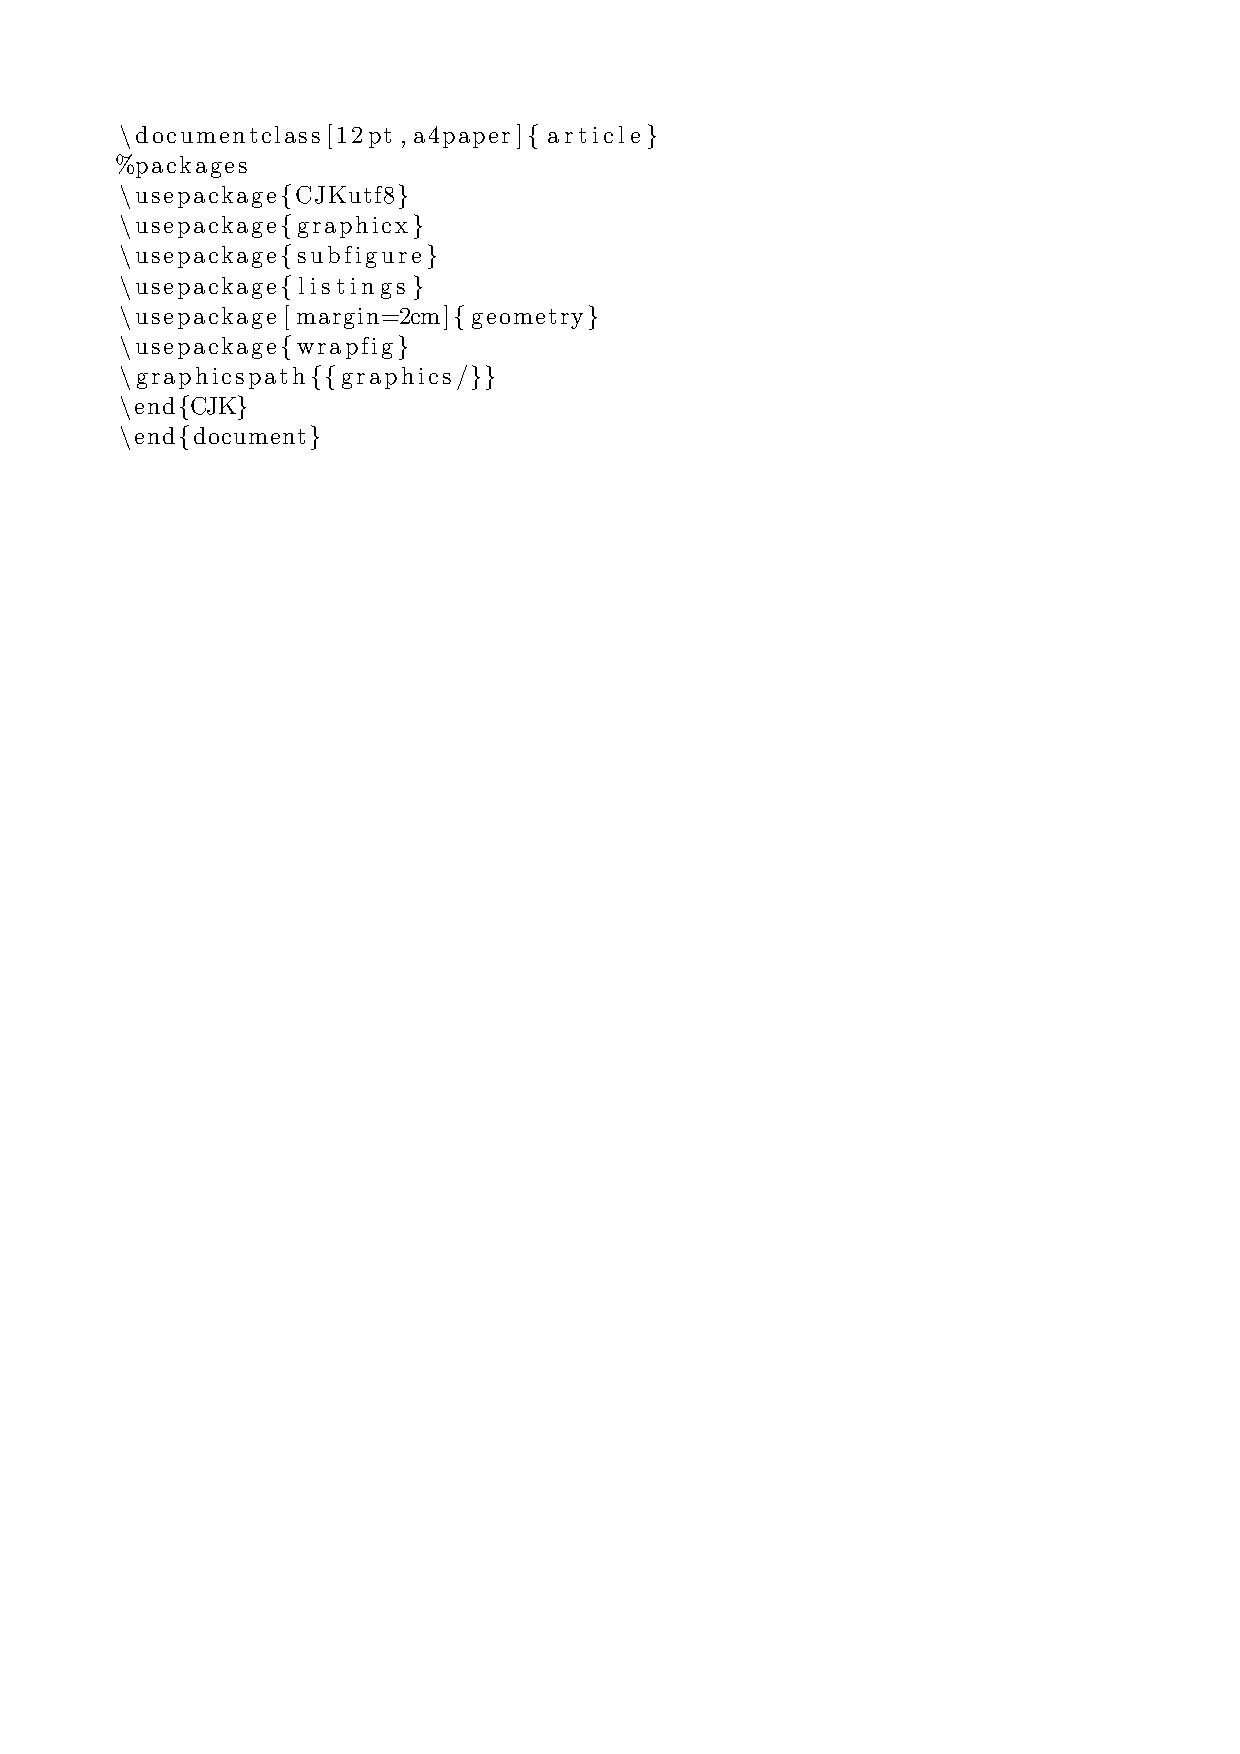
\includegraphics[scale=0.8]{./pics/setting.pdf}
\caption[es]{環境設定}
\label{ES}
\end{figure}
\begin{itemize}
\item \textcolor{red}{caption一定要用在label前面,否則會導致文章中呼叫圖片時無法顯示序號}
\end{itemize}


\section{Latex常用的圖片格式與命名原則}

\begin{itemize}
\item 點陣圖形:用格點的方式儲存資料,每一個格子是一個pixel,pixel數越高解析度就越高,可是在放大的時候會讓圖片產生鋸齒狀,導致影像失真。常用的圖檔格式:jpeg, gif, bmp, png, psd, tiff
\item 向量圖形:不是用格子的方式儲存,而是用每一點相對位置座標的方式儲存,放大或縮小時會重新計算,影像不會有失真的問題,但是需要的儲存空間較大。常見的圖檔格式:eps, pdf, svg
\item 一般為了避免圖形失真,建議使用向量圖形,matlab儲存檔案時可以直接將figure存成pdf檔案的格式,再匯入latex中可以避免圖形失真或是解析度過低
\item 命名原則:圖檔名字中間不可以有空格,否則會讀取不到,匯入時可以不用填寫副檔名
\end{itemize}

\newpage
\section{浮動位置}
\begin{itemize}
\item 範例一:沒有任何設定
\begin{figure}[!h] 
\begin{minipage}[b]{0.5\textwidth} 
\centering 
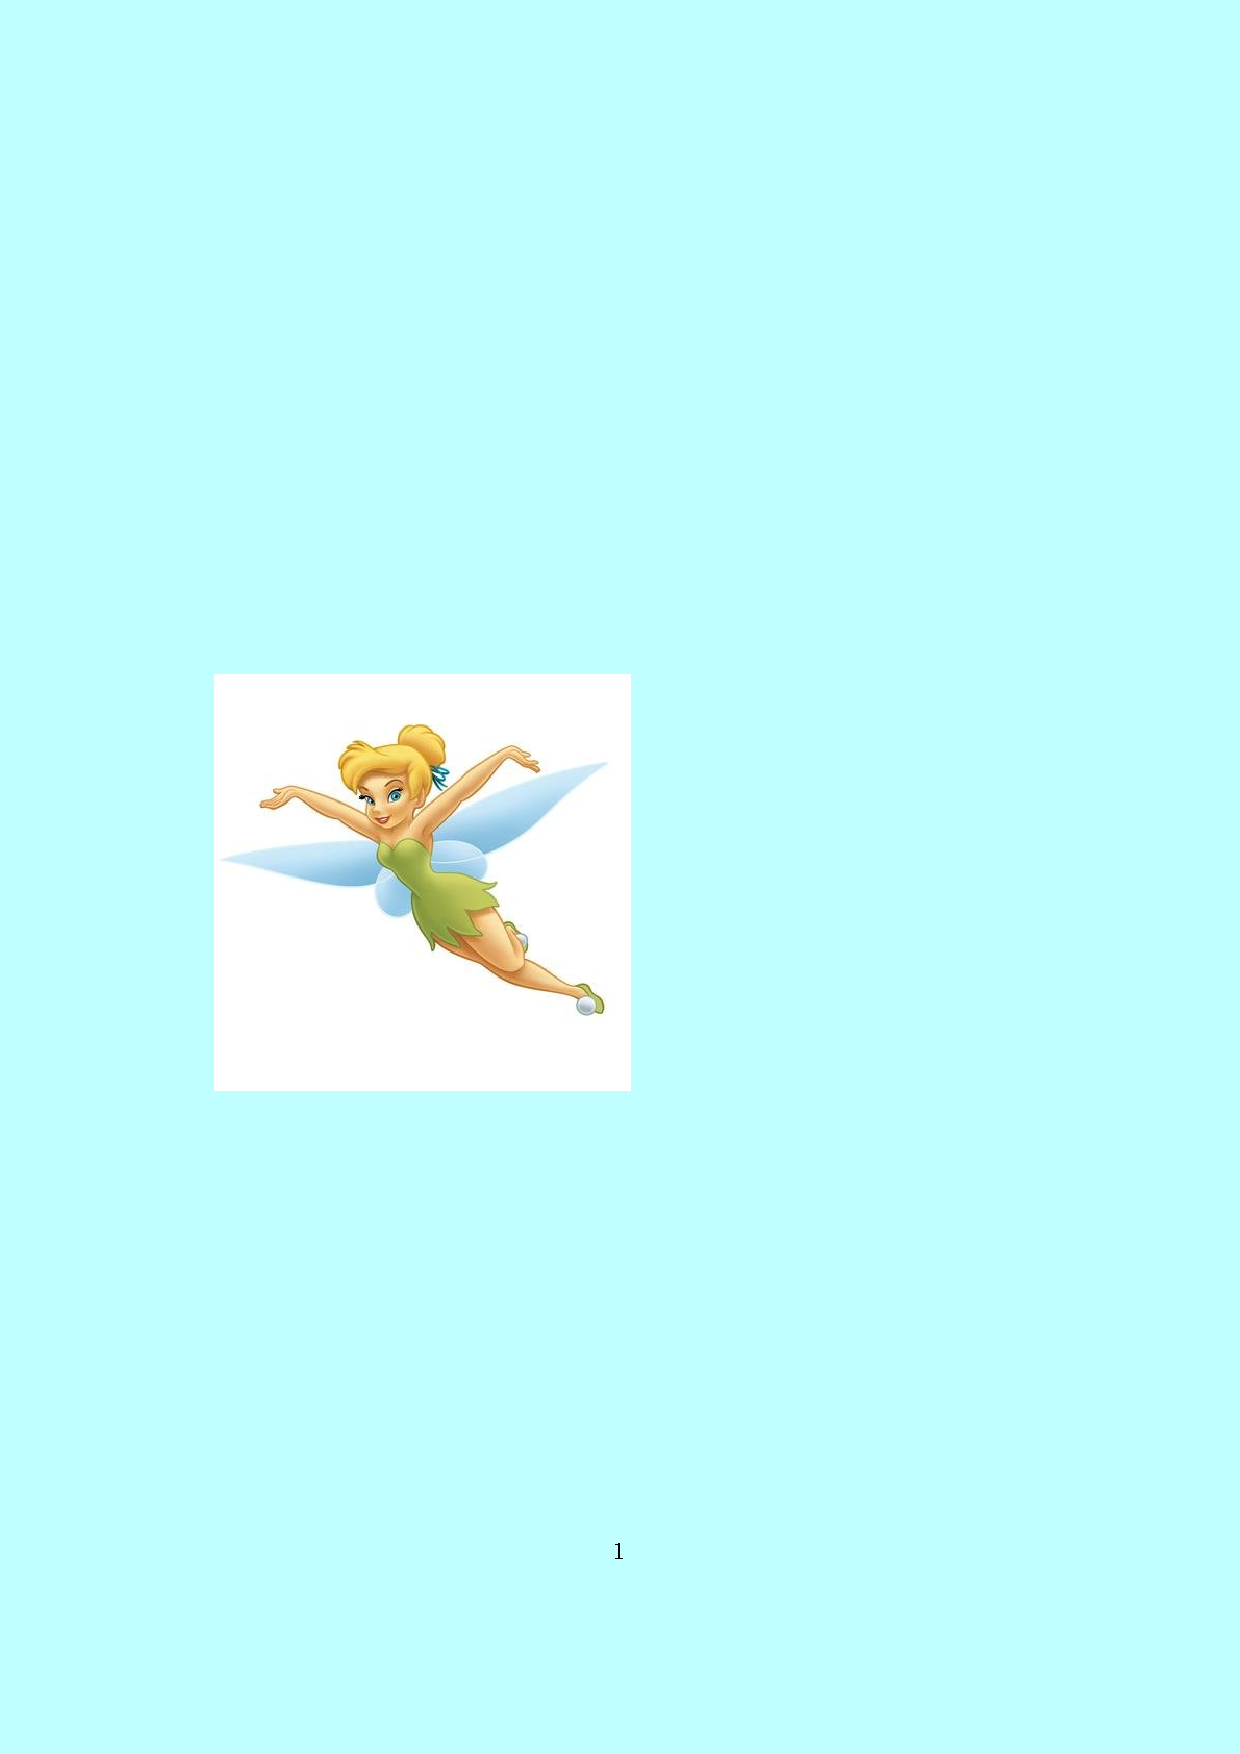
\includegraphics[scale=0.3]{./pics/float_example_1.pdf} 
\end{minipage}% 
\begin{minipage}[b]{0.5\textwidth} 
\begin{footnotesize}
\begin{quote}
\begin{verbatim}
\begin{figure}

\includegraphics[scale=0.5]{./pics/tinklebell.jpg}
\end{figure}
\end{verbatim}
\end{quote}
\end{footnotesize}
\end{minipage} 
\caption{浮動範例一}
\end{figure}

\item 範例二:設定為h,指定圖的位置在"這裡 (here)",圖顯示在哪裡會跟程式碼裡面圖與文字的相對位置有關係,範例中文字在圖之上,所以輸出也是文字在圖之上
\begin{figure}[!h] 
\begin{minipage}[b]{0.5\textwidth} 
\centering 
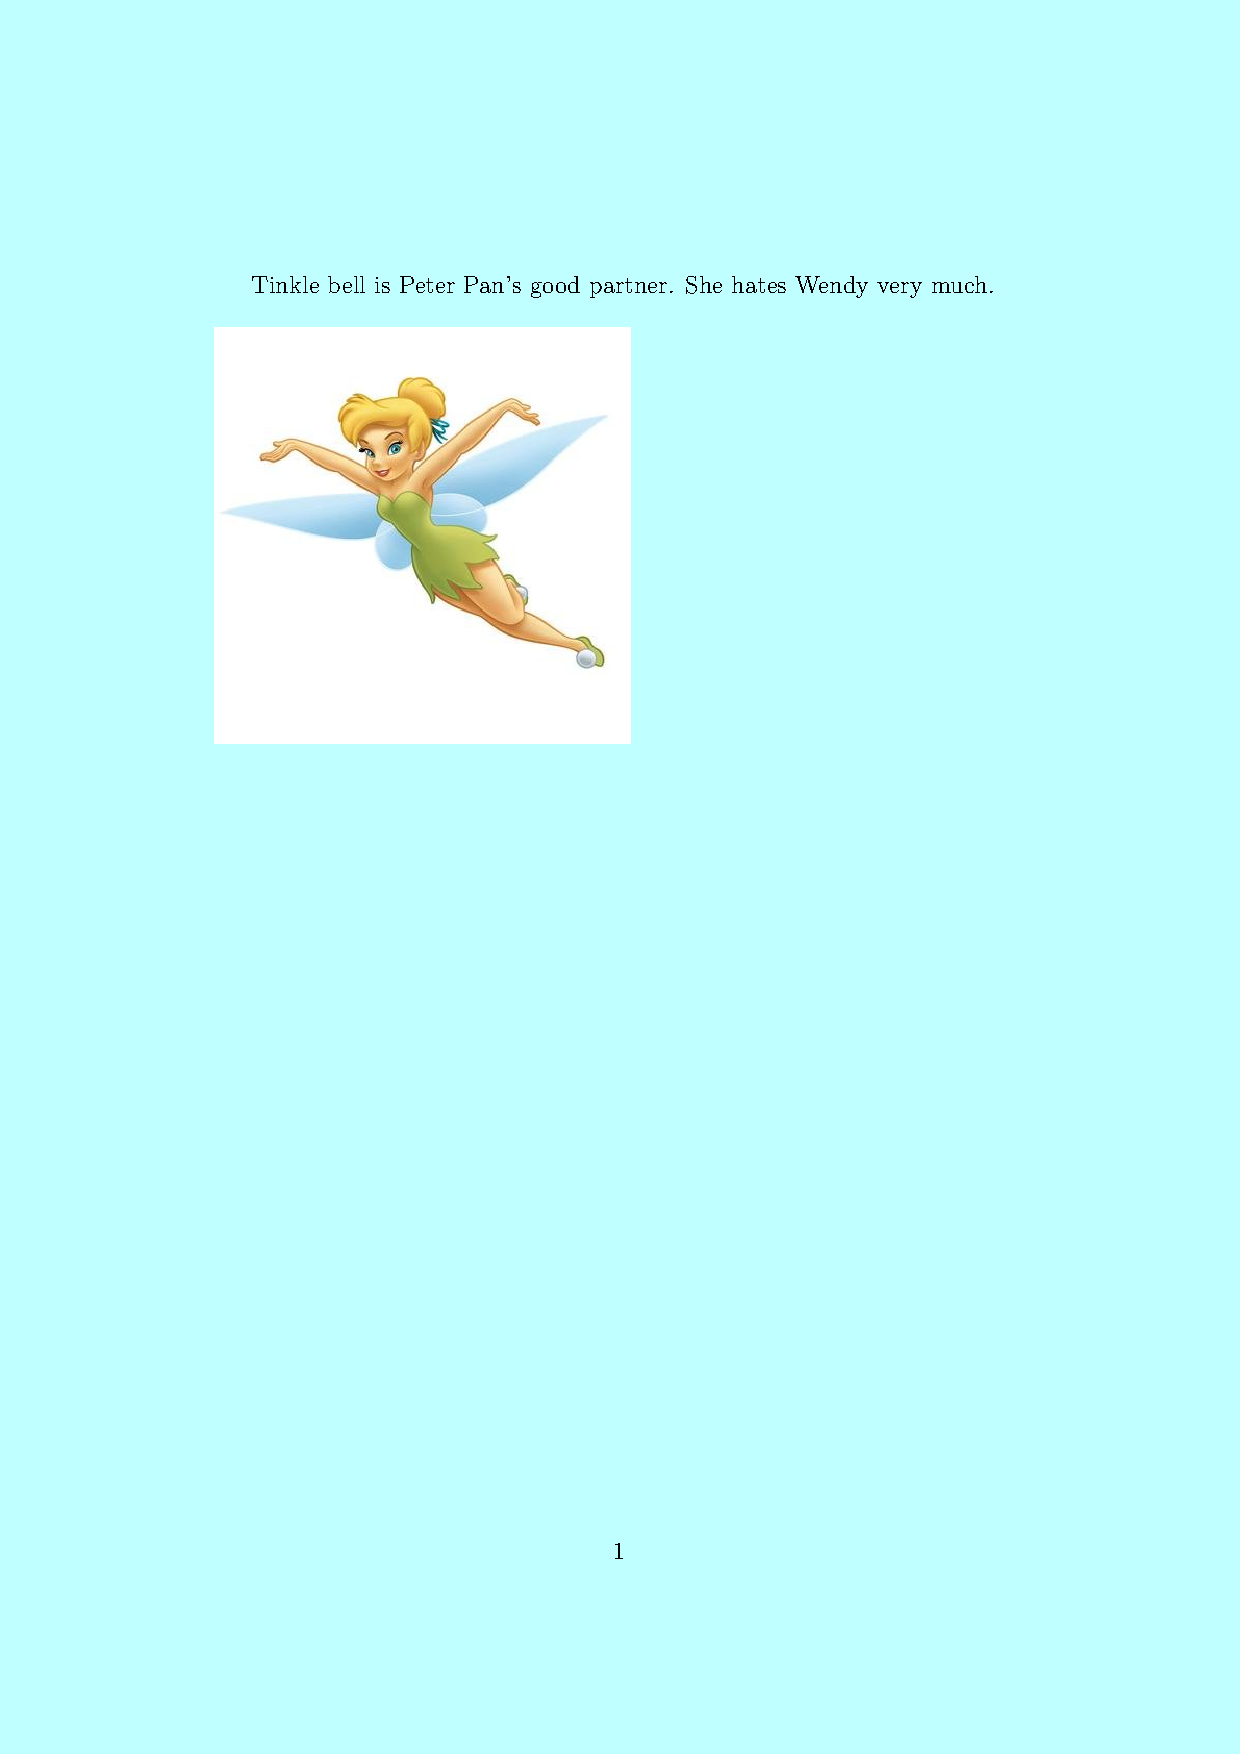
\includegraphics[scale=0.3]{./pics/float_example_7.pdf} 
\end{minipage}% 
\begin{minipage}[b]{0.5\textwidth} 
\begin{footnotesize}
\begin{quote}
\begin{verbatim}
Tinkle bell is Peter Pan's good partner. 
She hates Wendy very much
\begin{figure}[h]

\includegraphics[scale=0.5]{./pics/tinklebell.jpg}
\end{figure}
\end{verbatim}
\end{quote}
\end{footnotesize}
\end{minipage} 
\caption{浮動範例二}
\end{figure}

\item 範例三:設定為t,指定圖的位置在"上面 (top)",即使在程式碼裡面文字在圖之上,但是使用t代表圖要頁面的在上面,所以輸出結果是圖在文字之上
\begin{figure}[!h] 
\begin{minipage}[b]{0.5\textwidth} 
\centering 
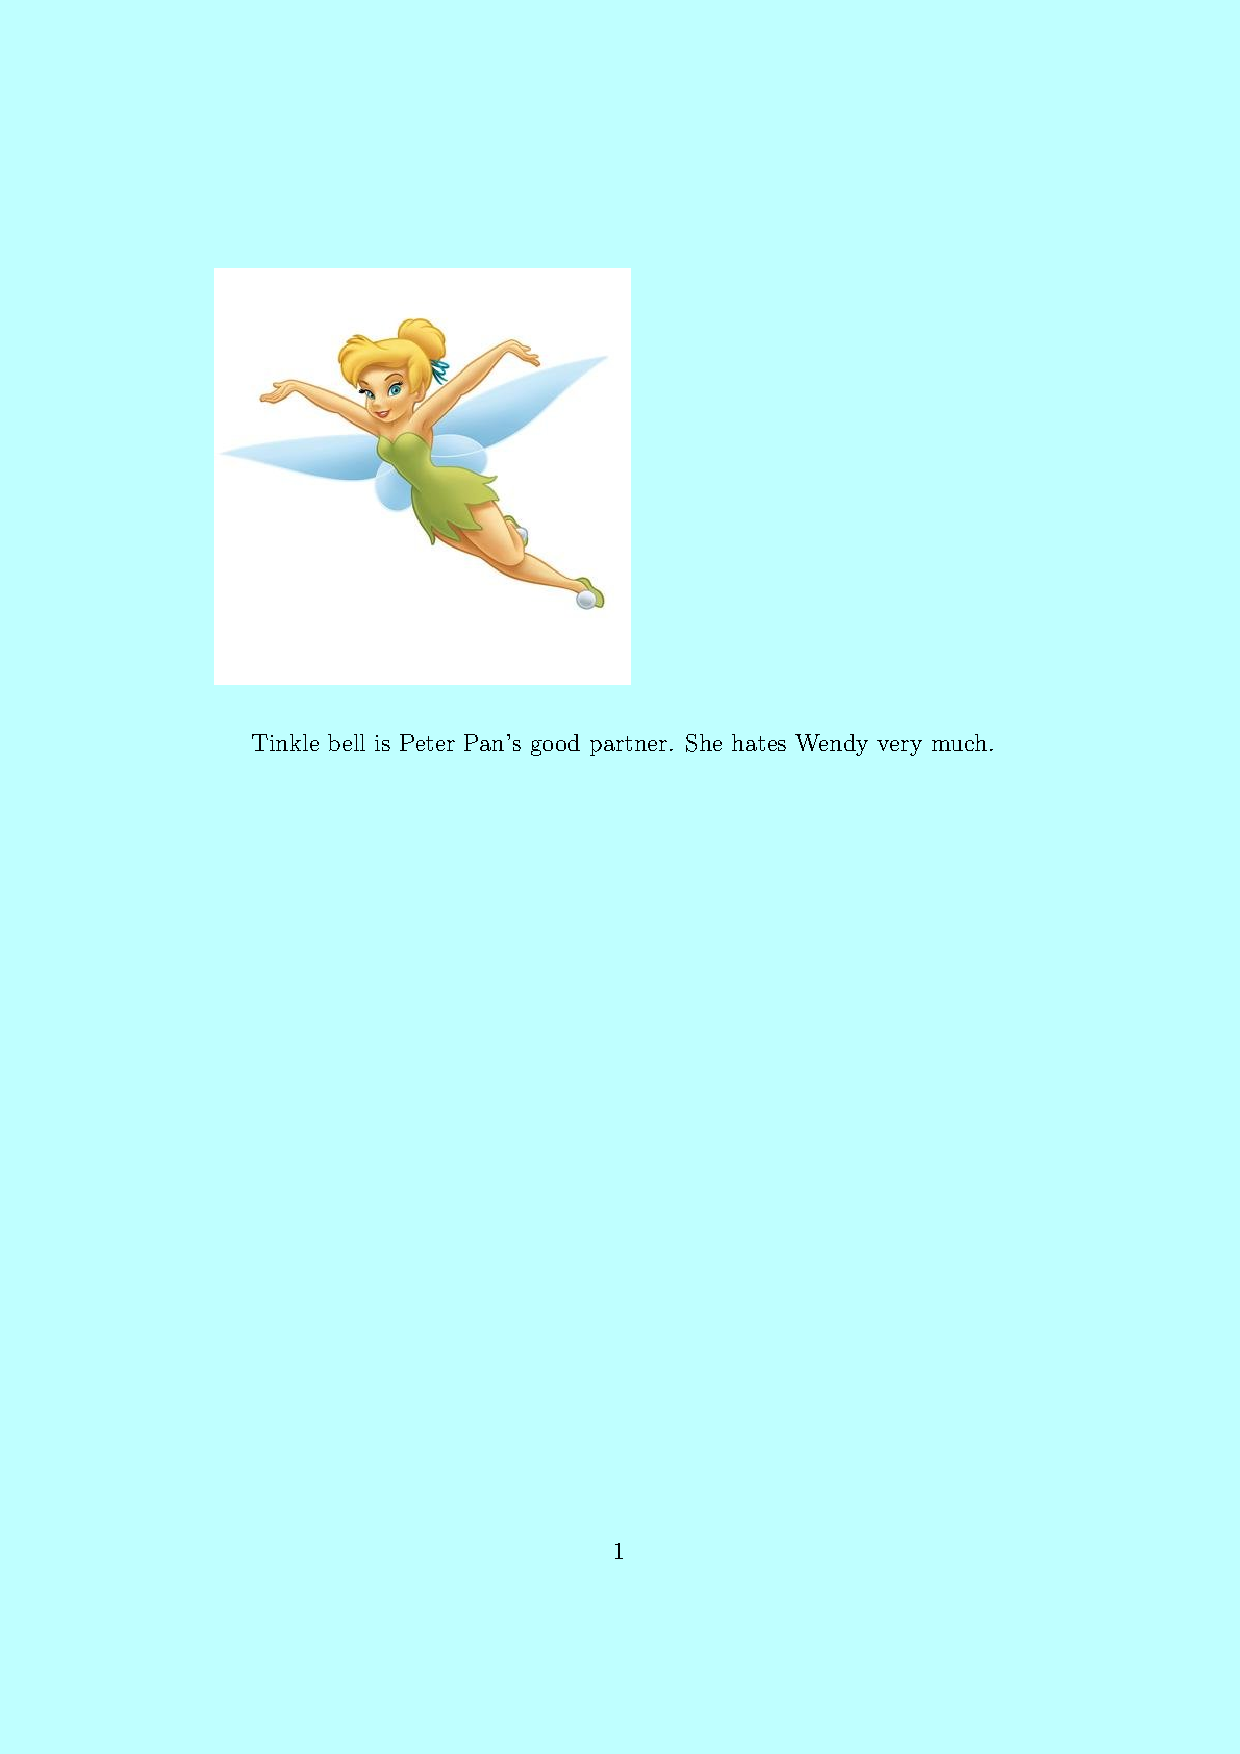
\includegraphics[scale=0.3]{./pics/float_example_9.pdf} 
\end{minipage}% 
\begin{minipage}[b]{0.5\textwidth} 
\begin{footnotesize}
\begin{quote}
\begin{verbatim}
Tinkle bell is Peter Pan's good partner. 
She hates Wendy very much.
\begin{figure}[t]

\includegraphics[scale=0.5]{./pics/tinklebell.jpg}
\end{figure}
\end{verbatim}
\end{quote}
\end{footnotesize}
\end{minipage} 
\caption{浮動範例三}
\end{figure}


\item 範例四:設定為b,指定圖的位置在"下面 (bottom)"
\begin{figure}[!h] 
\begin{minipage}[b]{0.5\textwidth} 
\centering 
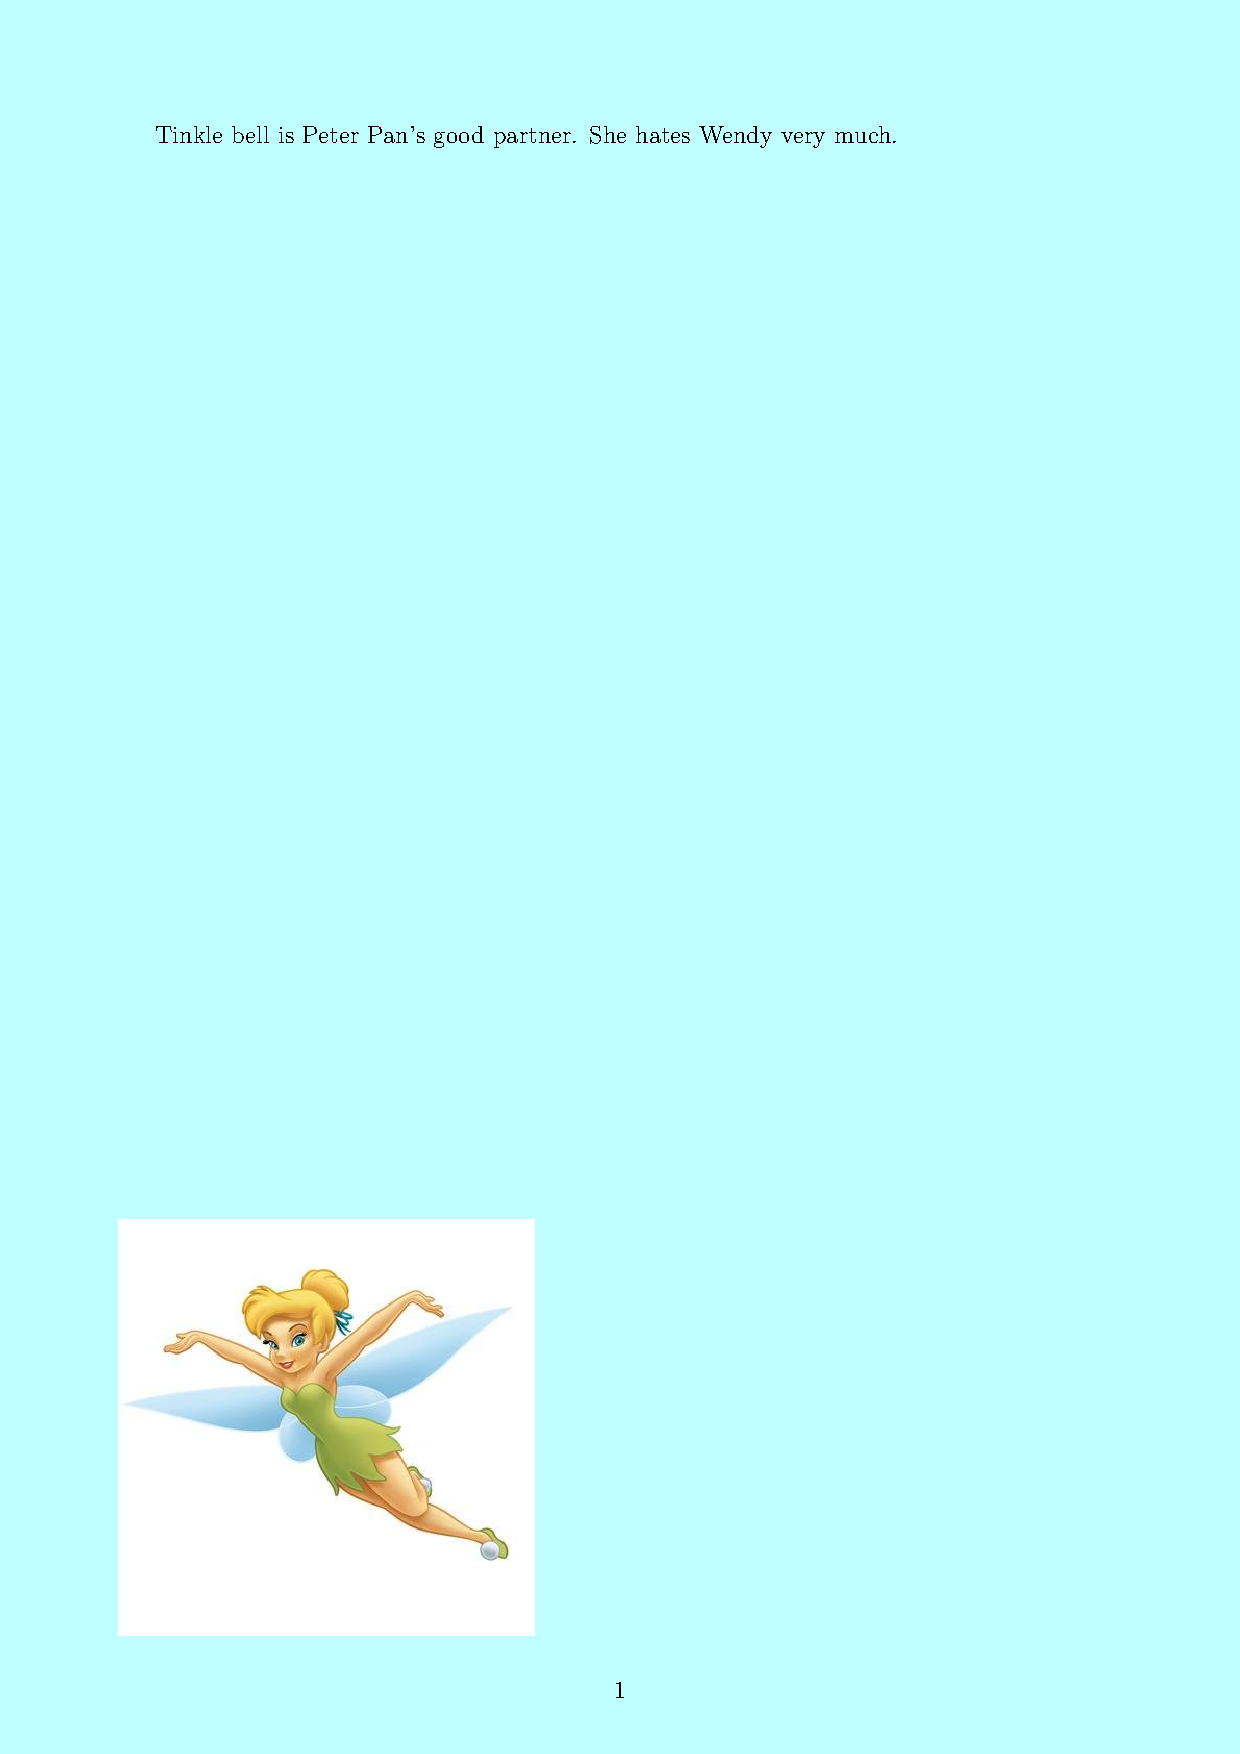
\includegraphics[scale=0.3]{./pics/float_example_10.pdf} 
\end{minipage}% 
\begin{minipage}[b]{0.5\textwidth} 
\begin{footnotesize}
\begin{quote}
\begin{verbatim}
Tinkle bell is Peter Pan's good partner. 
She hates Wendy very much
\begin{figure}[b]

\includegraphics[scale=0.5]{./pics/tinklebell.jpg}
\end{figure}
\end{verbatim}
\end{quote}
\end{footnotesize}
\end{minipage} 
\caption{浮動範例四}
\end{figure}

\newpage

\item 範例五:設定為p,指定圖的位置為浮動
\begin{figure}[!h] 
\begin{minipage}[b]{0.5\textwidth} 
\centering 
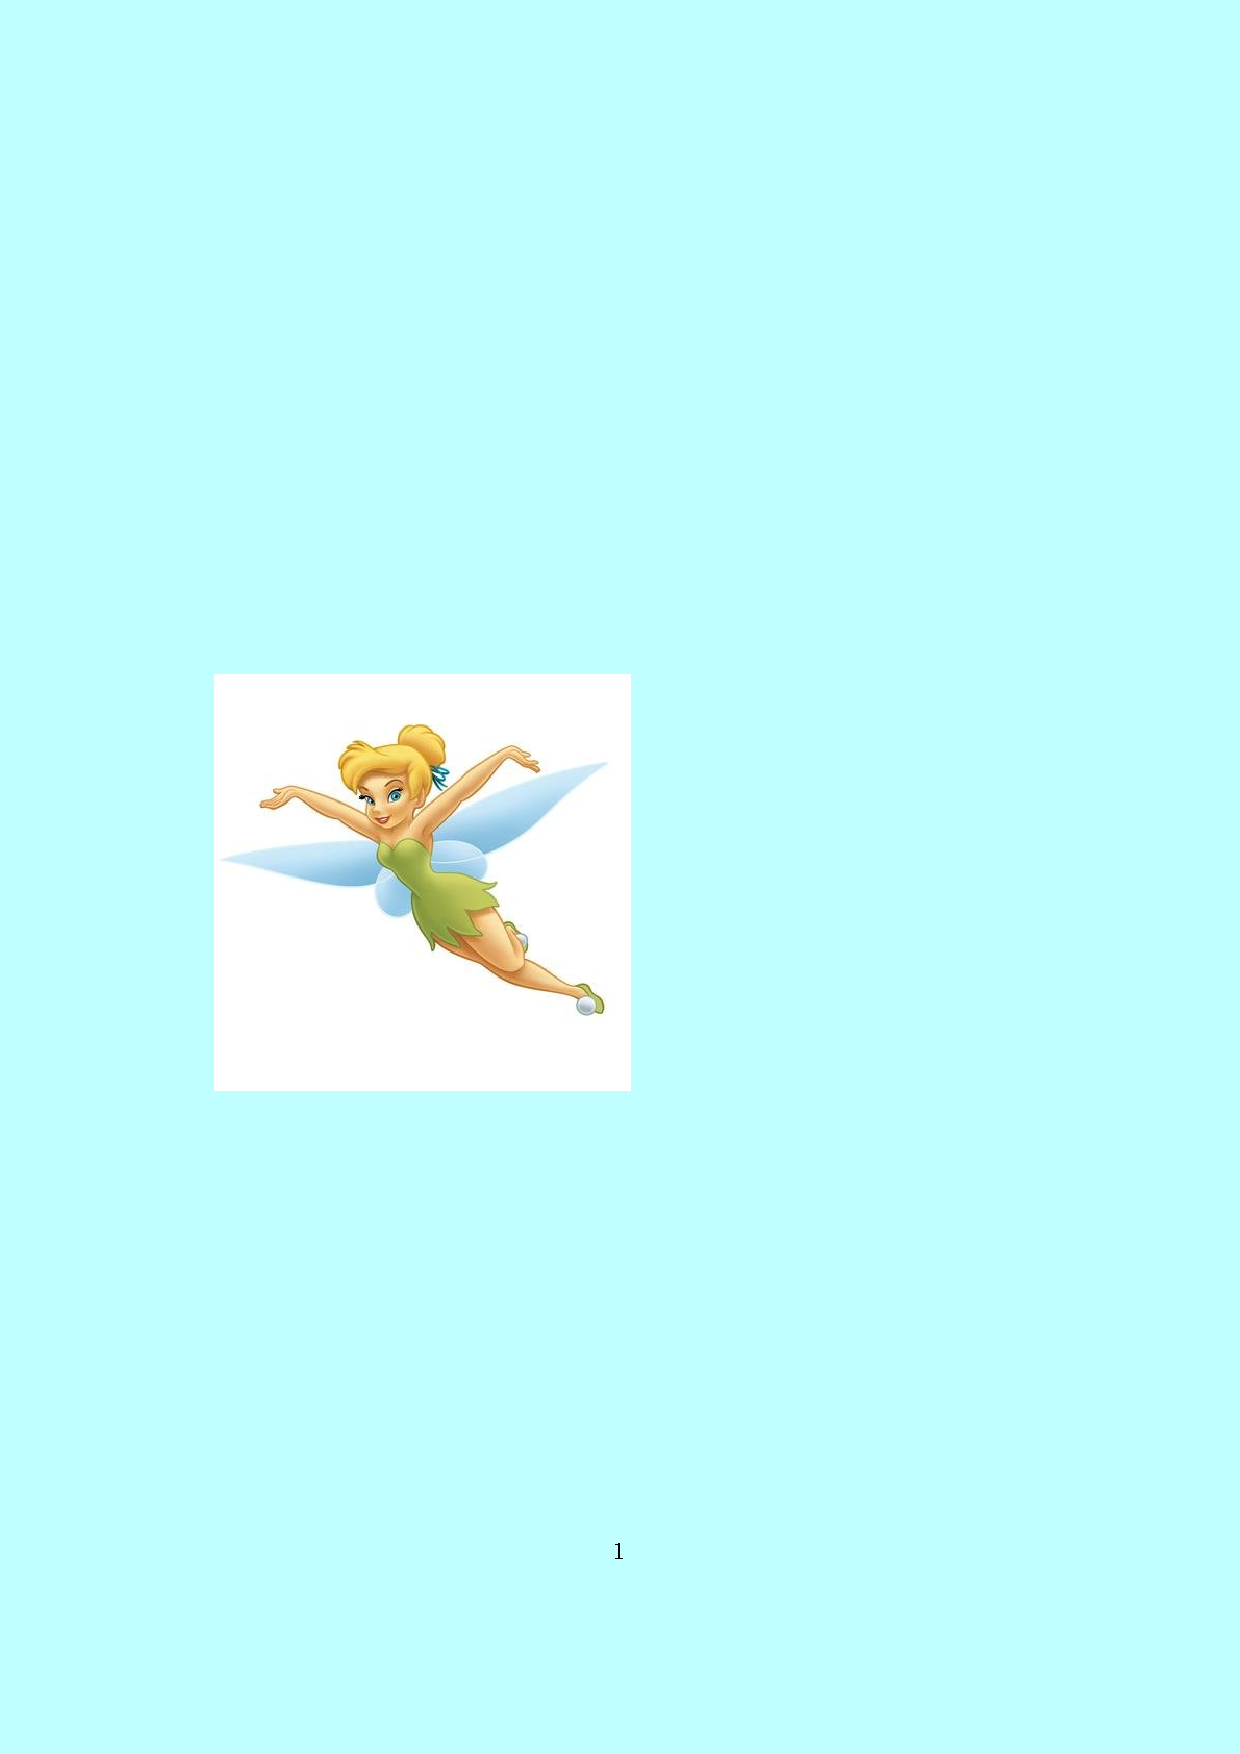
\includegraphics[scale=0.3]{./pics/float_example_3.pdf} 
\end{minipage}% 
\begin{minipage}[b]{0.5\textwidth} 
\begin{footnotesize}
\begin{quote}
\begin{verbatim}
\begin{figure}[p]

\includegraphics[scale=0.5]{./pics/tinklebell.jpg}
\end{figure}
\end{verbatim}
\end{quote}
\end{footnotesize}
\end{minipage} 
\caption{浮動範例五}
\end{figure}
\vspace{-0.5cm}
\item 因為圖片預設的位置都是浮動的,也就是說latex會幫圖片找到一個它覺得最合適的位置,如果想要控制圖片一定是在哪兩行文字之間,或是一定要在整個頁面的哪個位置的話,可以在htb前面加上驚嘆號,[!h]為固定在這裡,[!b]為強制在整個頁面的最下面,[!t]為強制在整個頁面的最上面
\end{itemize}

\vspace{-1cm}
\section{圖片尺寸設定}
\vspace{-0.5cm}
\begin{figure}[!h] 
\begin{minipage}[b]{0.5\textwidth} 
\centering 
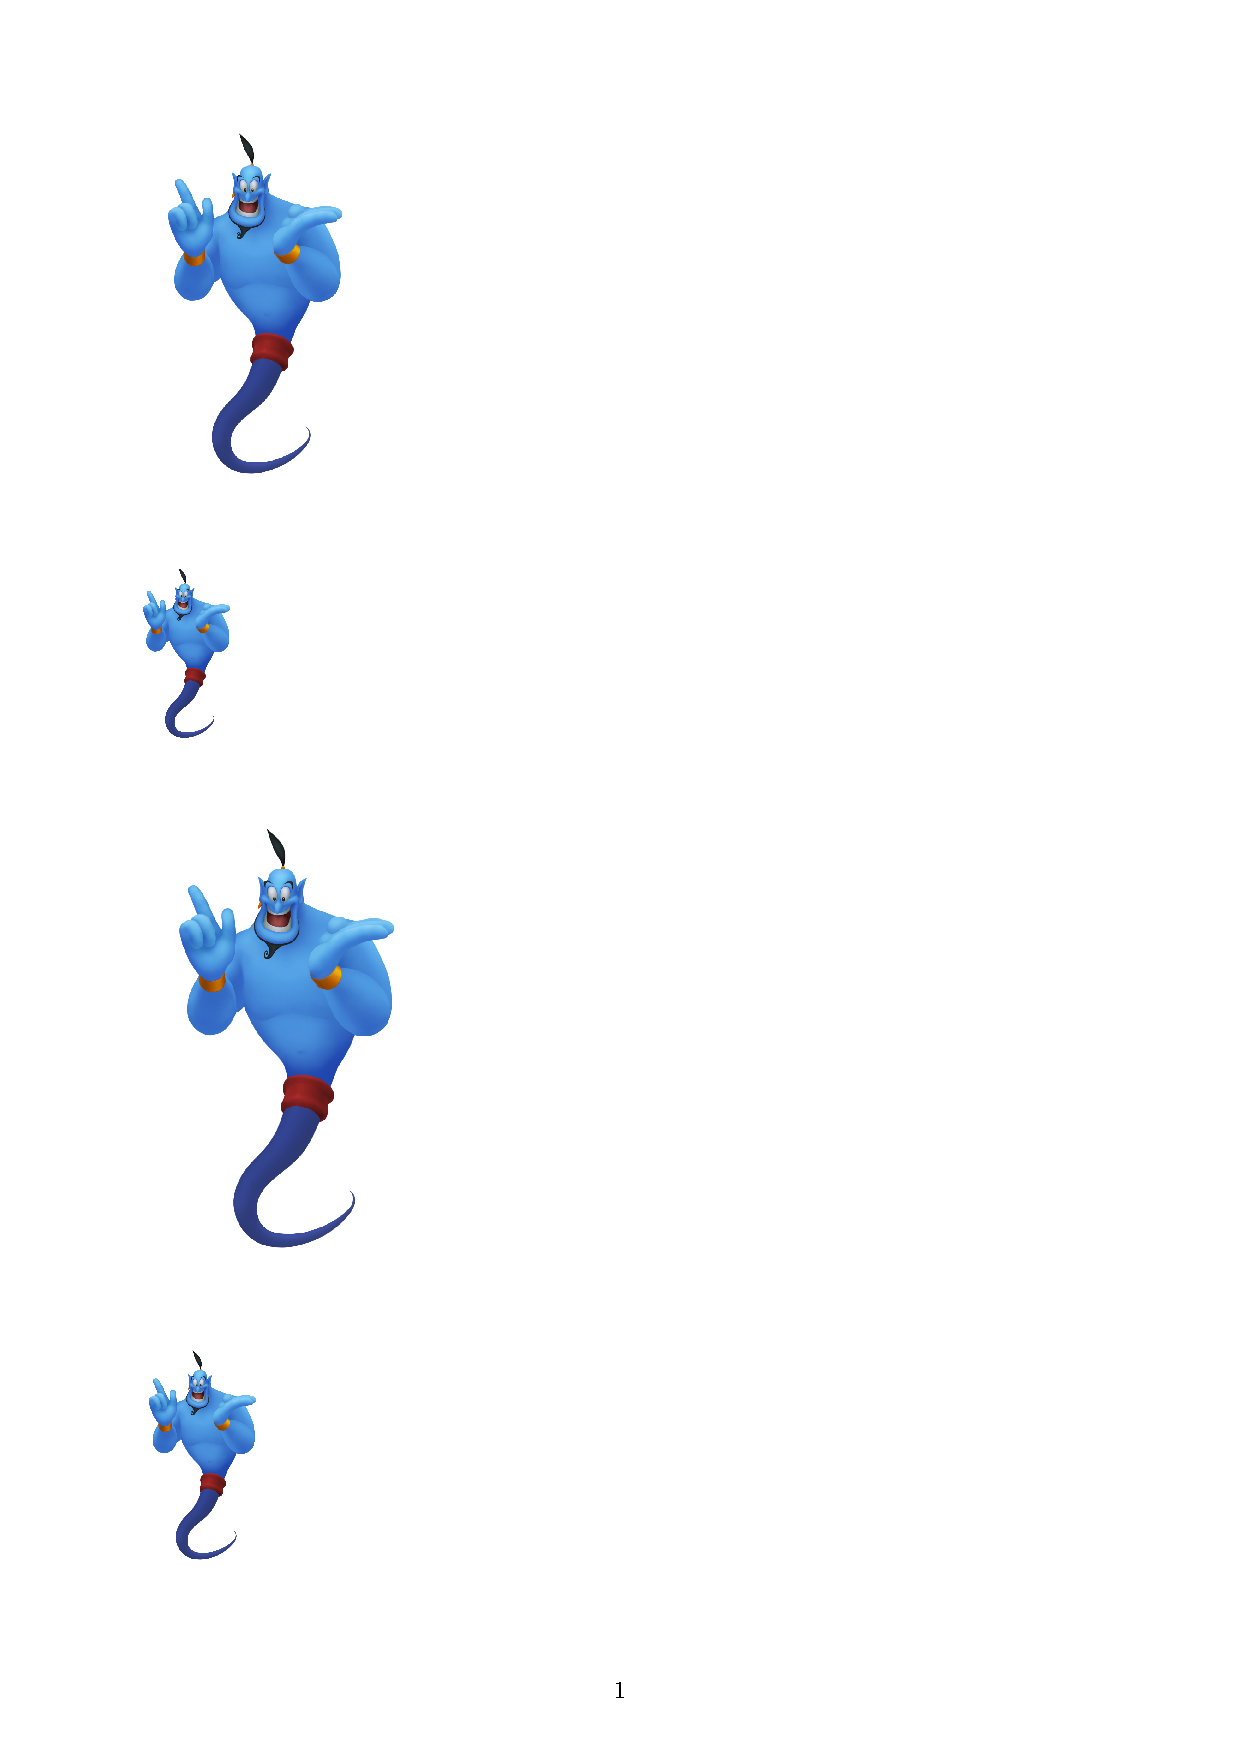
\includegraphics[scale=0.3]{./pics/size_example.pdf} 
\end{minipage}% 
\begin{minipage}[b]{0.5\textwidth} 
\begin{footnotesize}
\begin{quote}
\begin{verbatim}
\begin{figure}[!h]

\includegraphics{./pics/genie.jpg}
\end{figure}
\begin{figure}[!h]

\includegraphics[scale=0.5]{./pics/genie.jpg}
\end{figure}
\begin{figure}[!h]

\includegraphics[width=6cm]{./pics/genie.jpg}
\end{figure}
\begin{figure}[!h]

\includegraphics[height=4cm]{./pics/genie.jpg}
\end{figure}
\end{verbatim}
\end{quote}
\end{footnotesize}
\end{minipage} 
\caption{尺寸設定範例}
\end{figure}

\newpage
\section{Trim的用法}
\noindent 雖然可以利用圖形編輯軟體事先把圖片都調整到想要的尺寸之後再匯入文章中,不過有時候相同的東西要一張一張調也是挺麻煩的,尤其是matlab存成pdf檔案之後會有很多不想要的白邊,這時候就可以利用trim來把白邊剪掉,trim共要設定四個參數,代表想要檢調的左邊 下面 右邊 上面想要剪去的尺寸,如果只是想要把左邊的3公分剪掉,那麼就利用"trim=3cm 0cm 0cm 0cm,clip"就可以了,感謝子頡學長提供裁剪matlab輸出神秘參數"[trim=1.5cm 6.5cm 1.5cm 8.5cm]"。備註:這個方法只能用在裁切pdf檔案,一般圖檔無法使用。
\begin{footnotesize}
\begin{quote}
\begin{verbatim}
\begin{figure}[!h]
\centering
\subfigure[裁切前]{
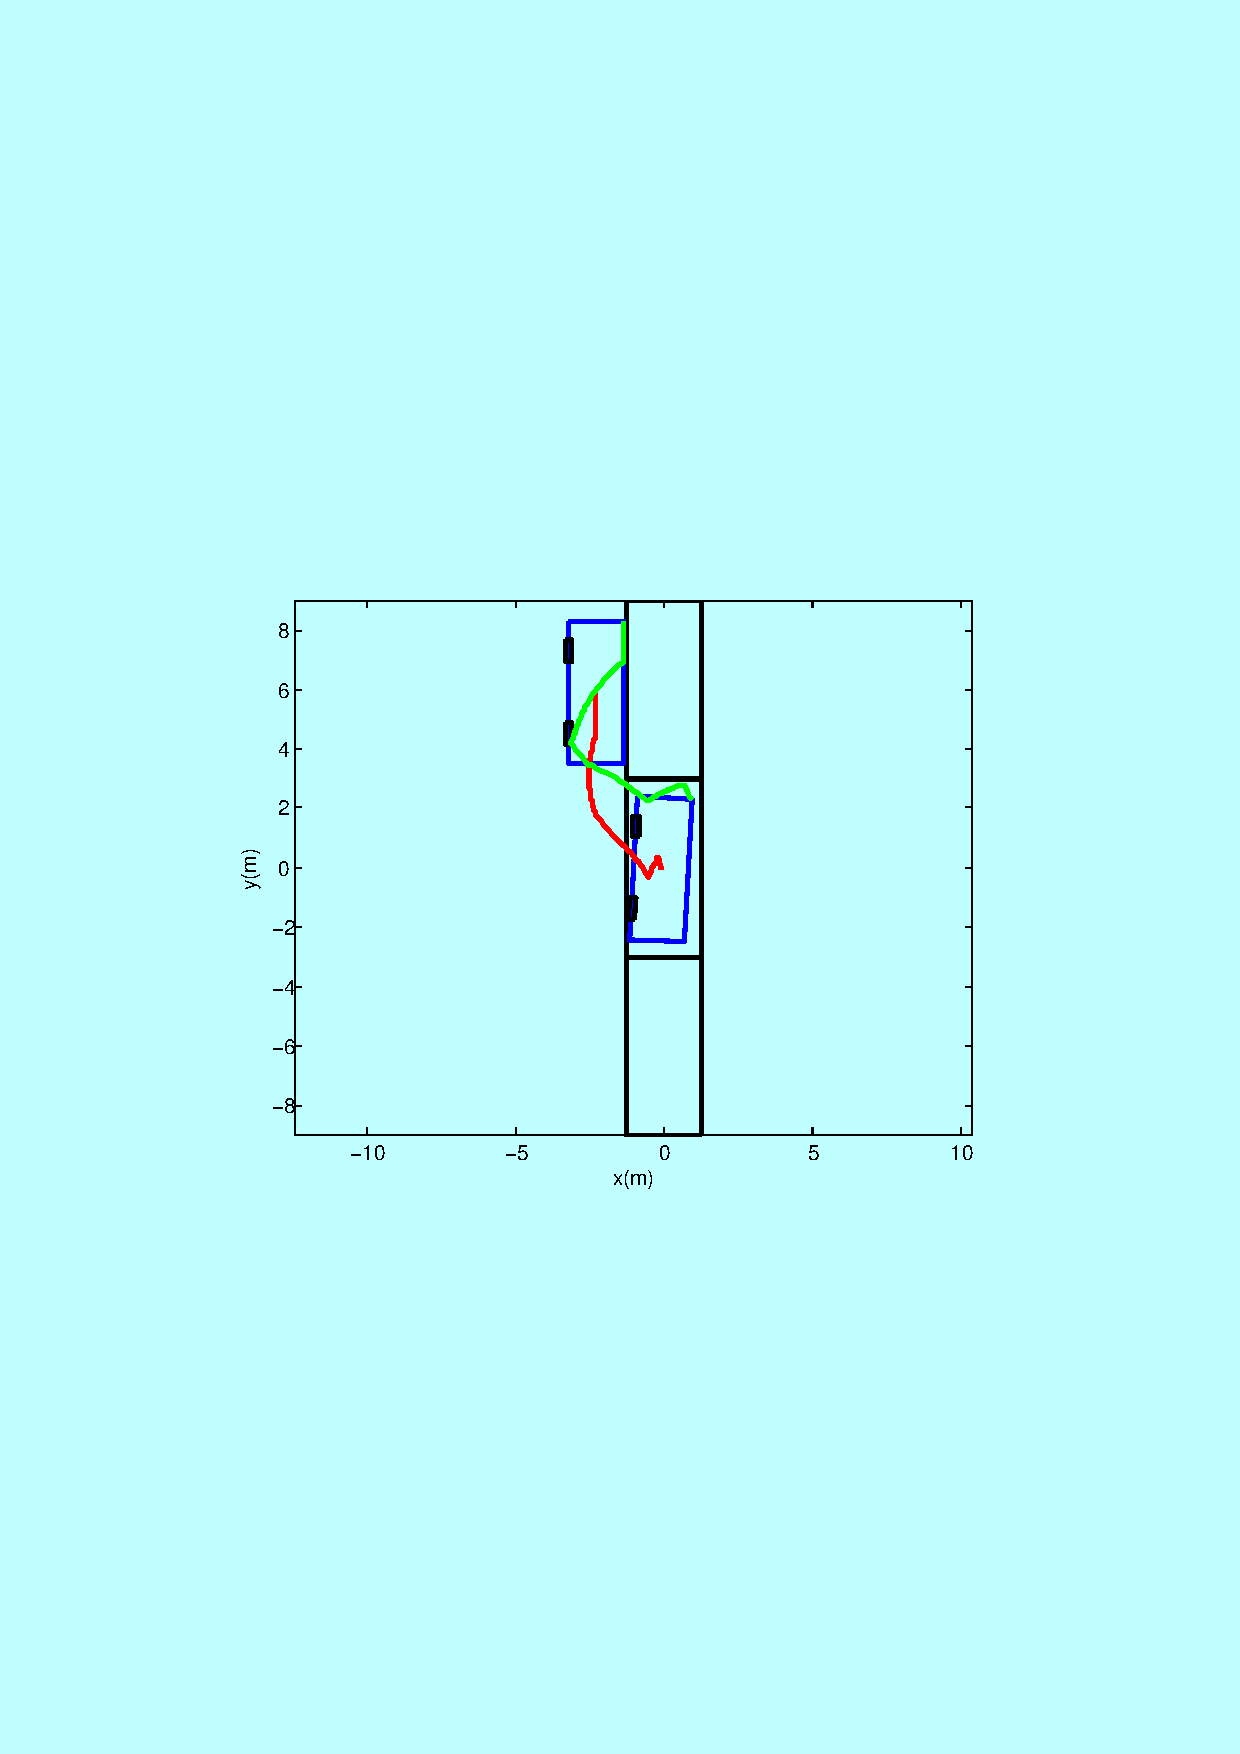
\includegraphics[scale=0.3]{./pics/matlab_example.pdf}}
\subfigure[裁切後]{
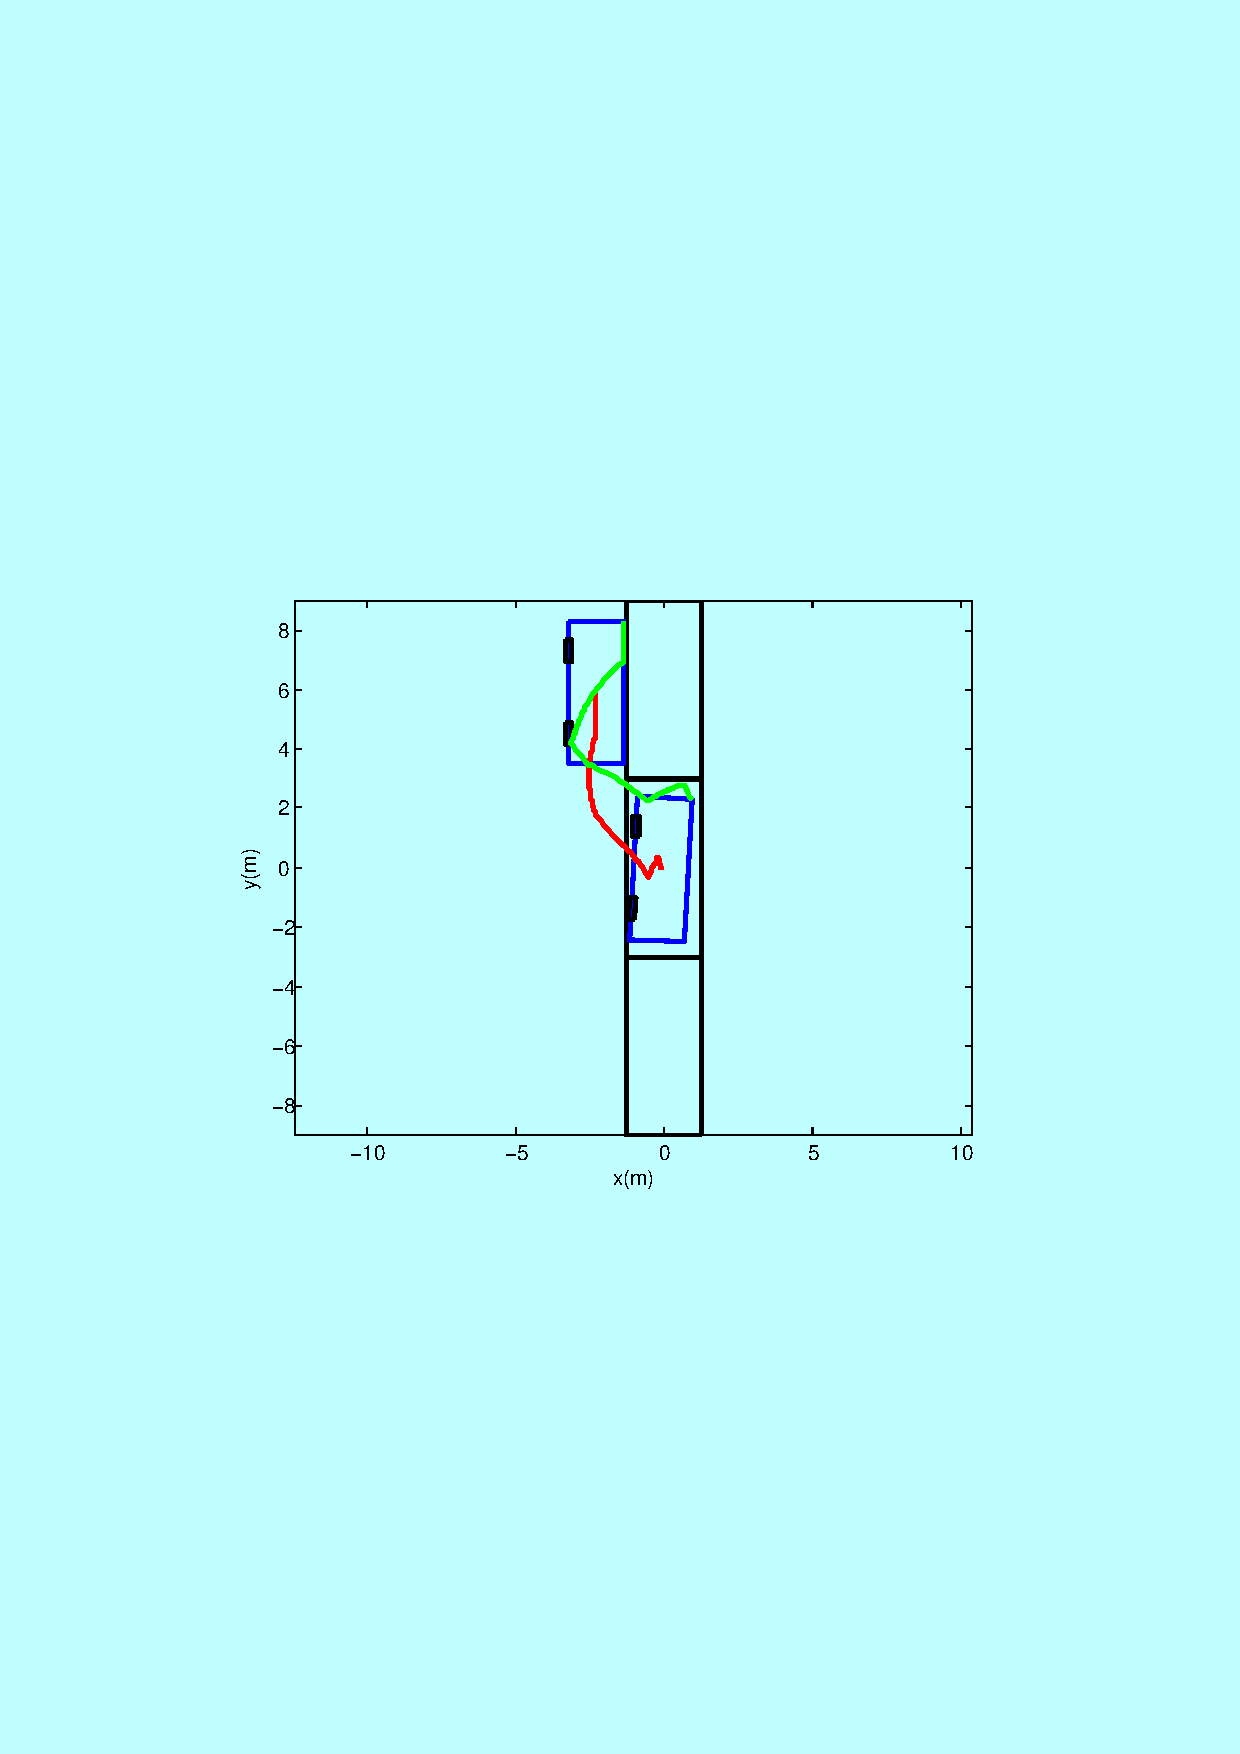
\includegraphics[trim=1.5cm 6.5cm 1.5cm 8.5cm,clip,scale=0.3]{./pics/matlab_example.pdf}}
\end{figure}
\end{verbatim}
\end{quote}
\end{footnotesize}
\vspace{-0.5cm}
\begin{figure}[!h]
\centering
\subfigure[裁切前]{
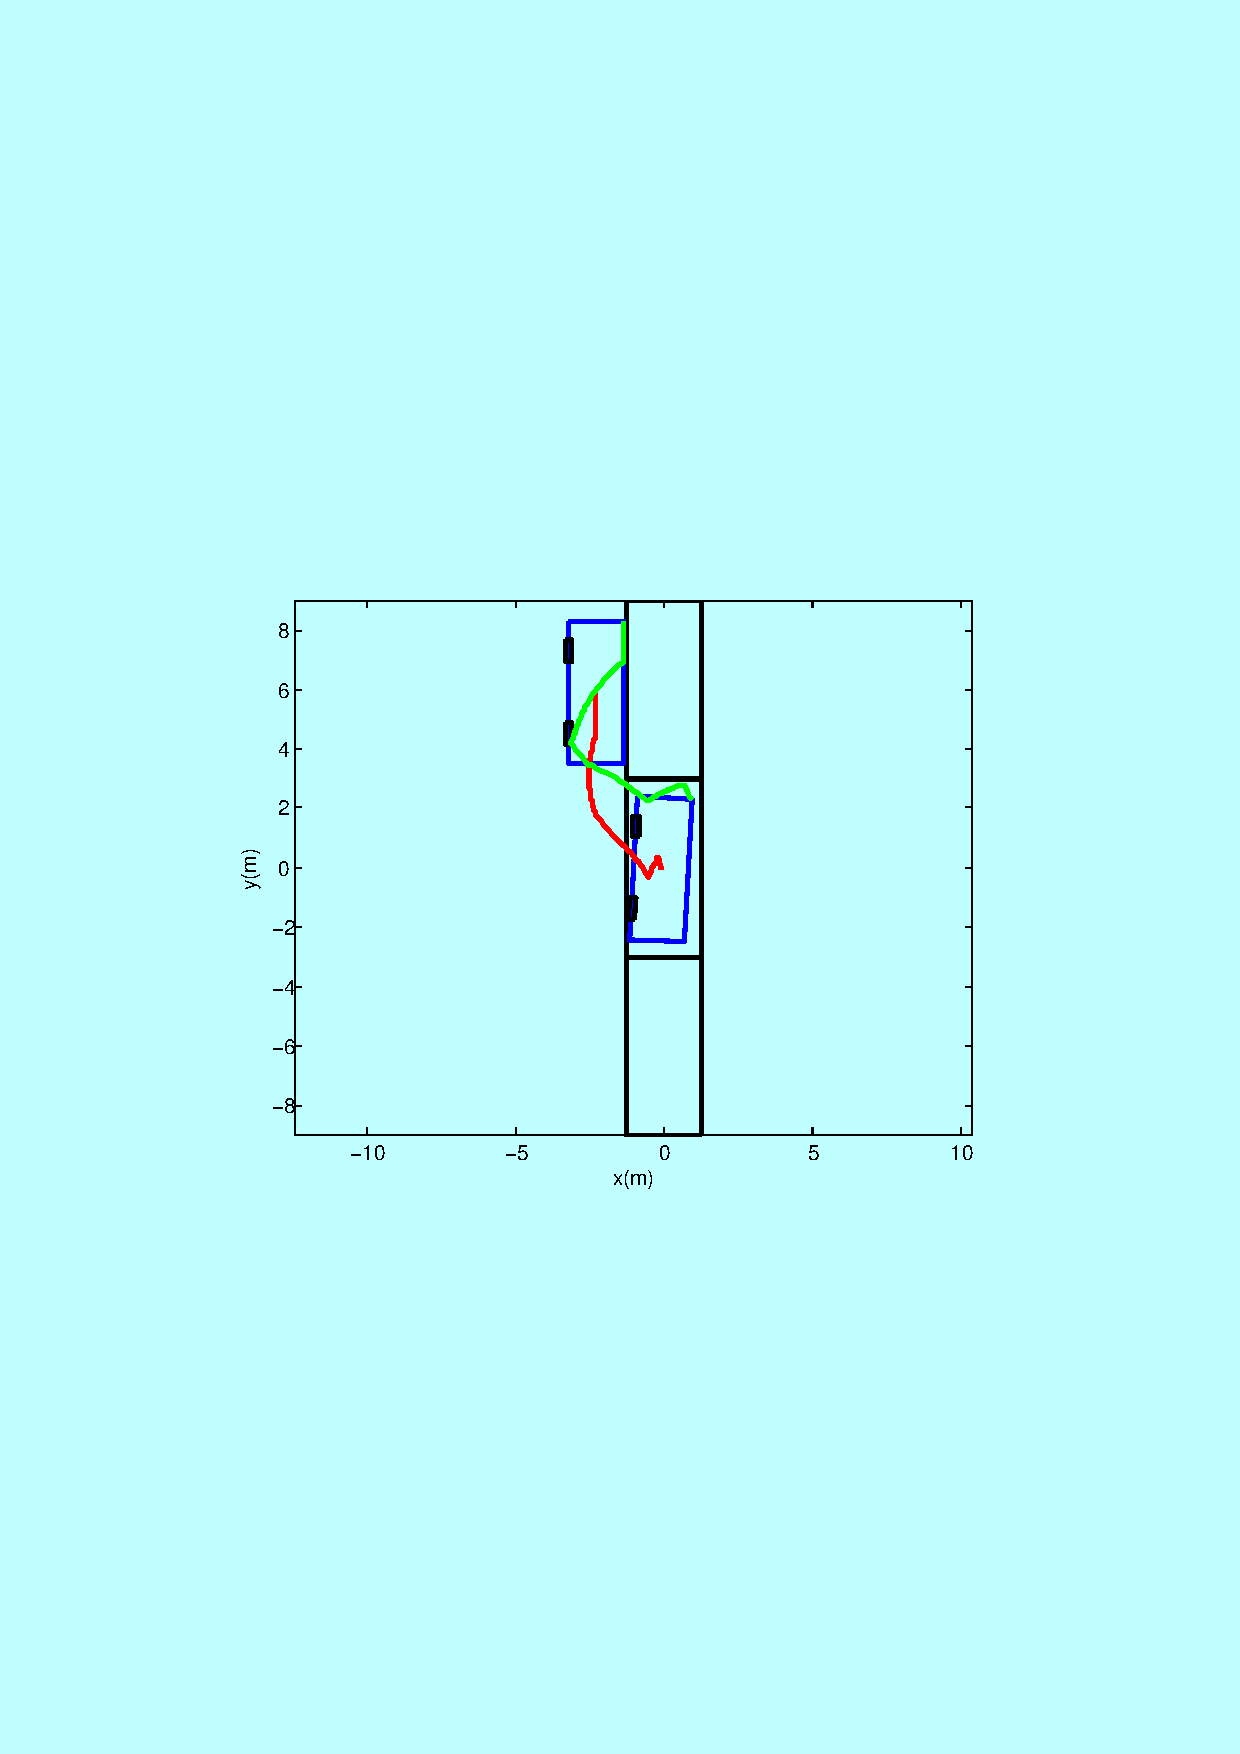
\includegraphics[scale=0.3]{./pics/matlab_example.pdf}}
\subfigure[裁切後]{
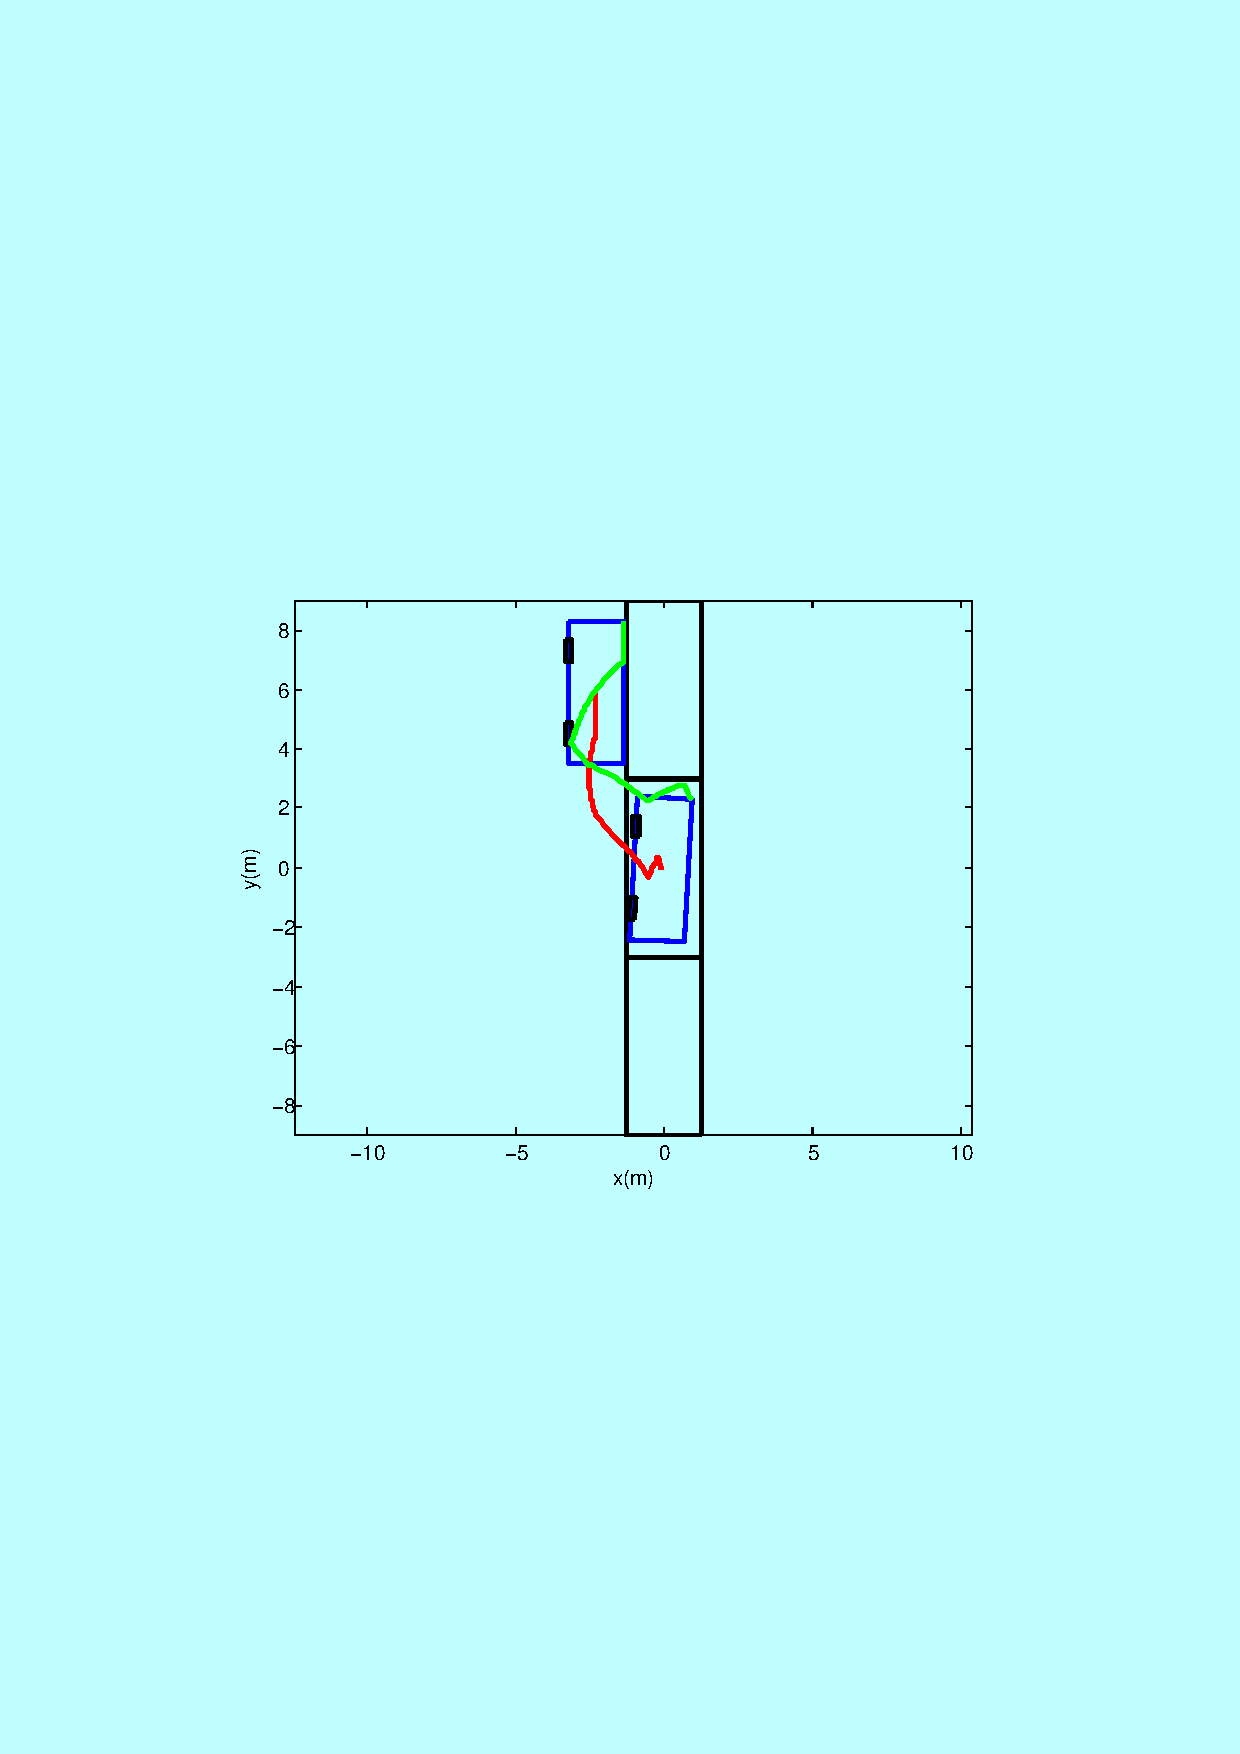
\includegraphics[trim=1.5cm 6.5cm 1.5cm 8.5cm,clip,scale=0.3]{./pics/matlab_example.pdf}}
\caption{trim 範例}
\end{figure}

\vspace{-1cm}
\section{Subfigure}
\vspace{-0.5cm}
\begin{figure}[!h] 
\begin{minipage}[b]{0.5\textwidth} 
\centering 
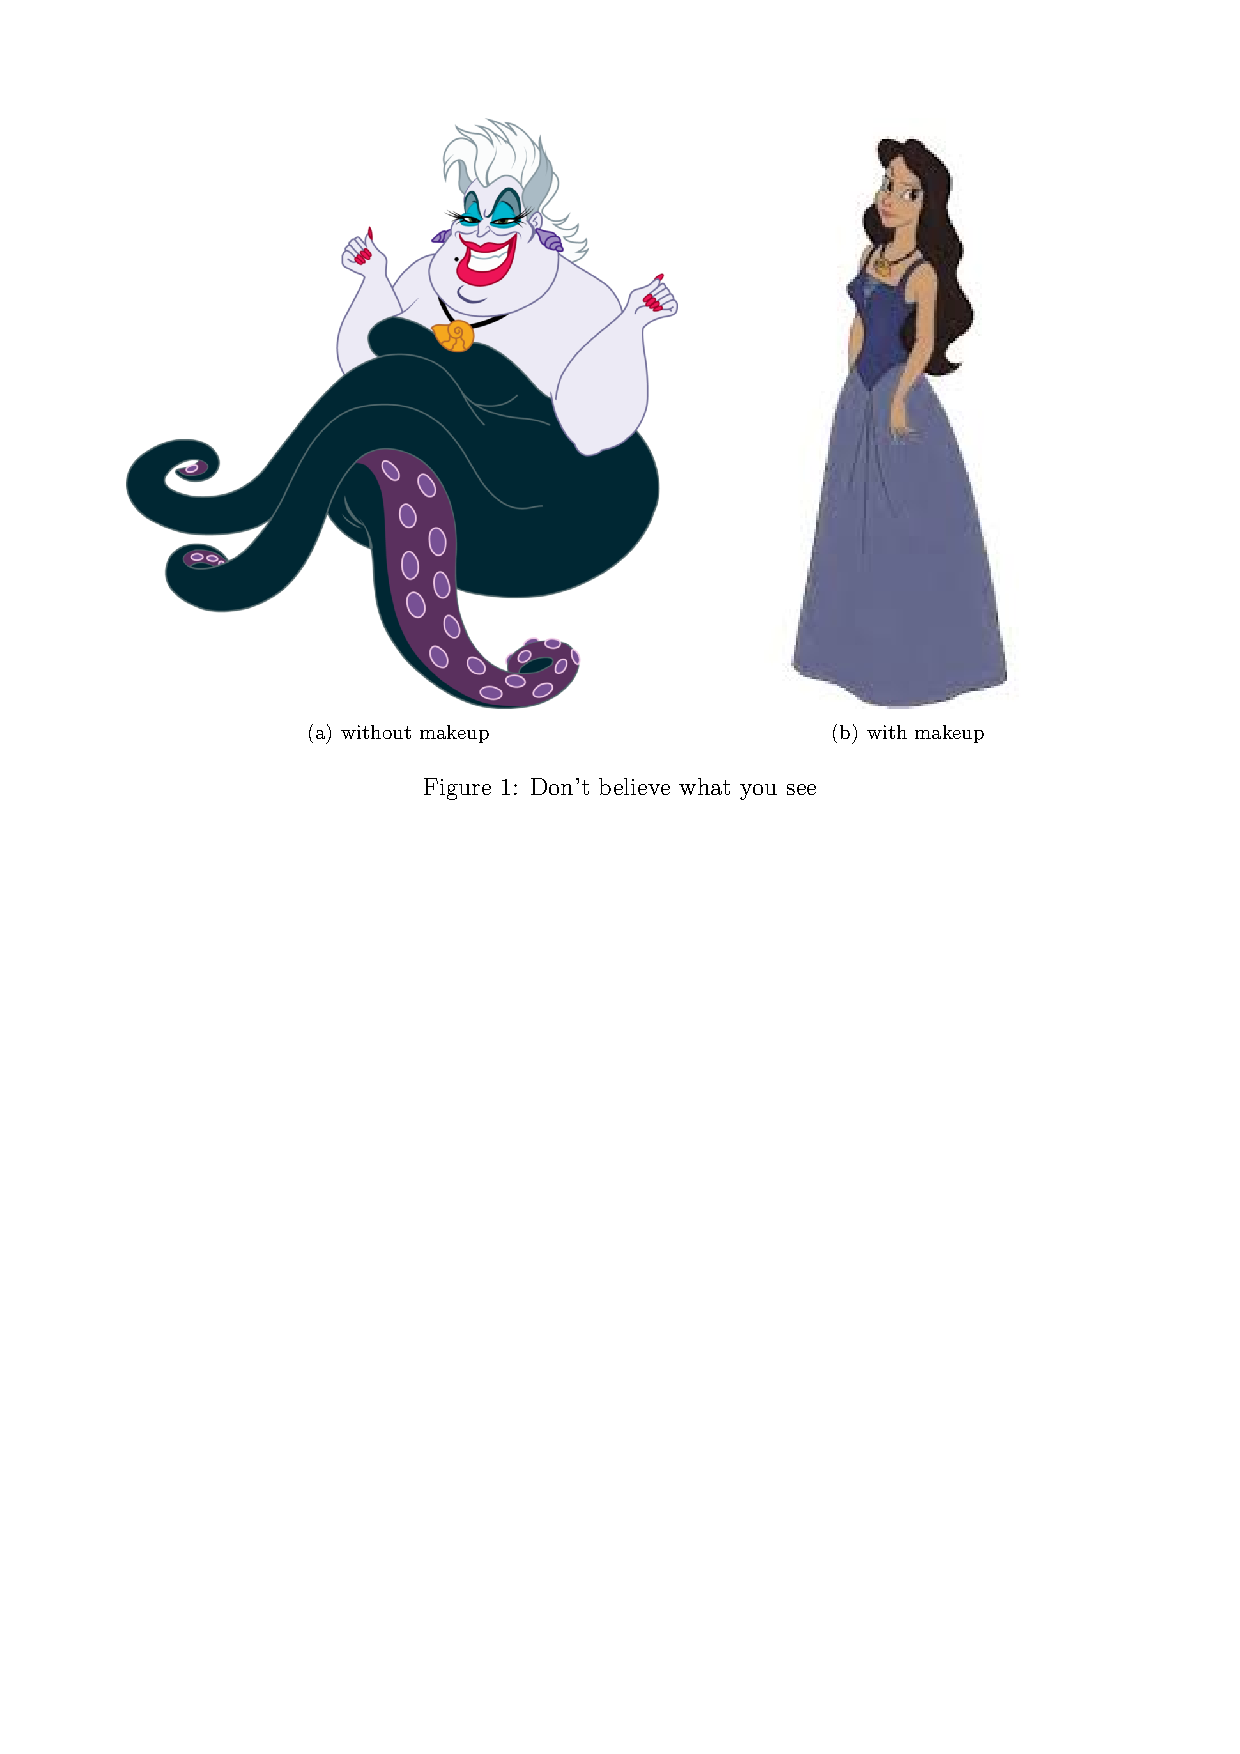
\includegraphics[scale=0.3]{./pics/subfigure_example.pdf} 
\end{minipage}% 
\begin{minipage}[b]{0.5\textwidth} 
\begin{footnotesize}
\begin{quote}
\begin{verbatim}
\begin{figure}[!h]
\subfigure[without makeup]{

\includegraphics[height=10cm]{./pics/ursula_before.png}}
\subfigure[with makeup]{

\includegraphics[height=10cm]{./pics/ursula_after.jpg}}
\caption{Don't believe what you see}
\end{figure}
\end{verbatim}
\end{quote}
\end{footnotesize}
\end{minipage} 
\caption{subfigure範例}
\end{figure}

\chapter{疑惑解答篇}
\vspace{-1cm}
\section{文繞圖}
\vspace{-0.5cm}
需要先引入wrapfig package,使用方法很簡單,可以利用r或是l調整圖在文字的哪一邊,在"\textbackslash end\{wrapfigure\}"下方加上``\textbackslash mbox\{\}"可以避免圖跟文字重疊

\begin{figure}[!h] 
\begin{minipage}[b]{0.5\textwidth} 
\centering 
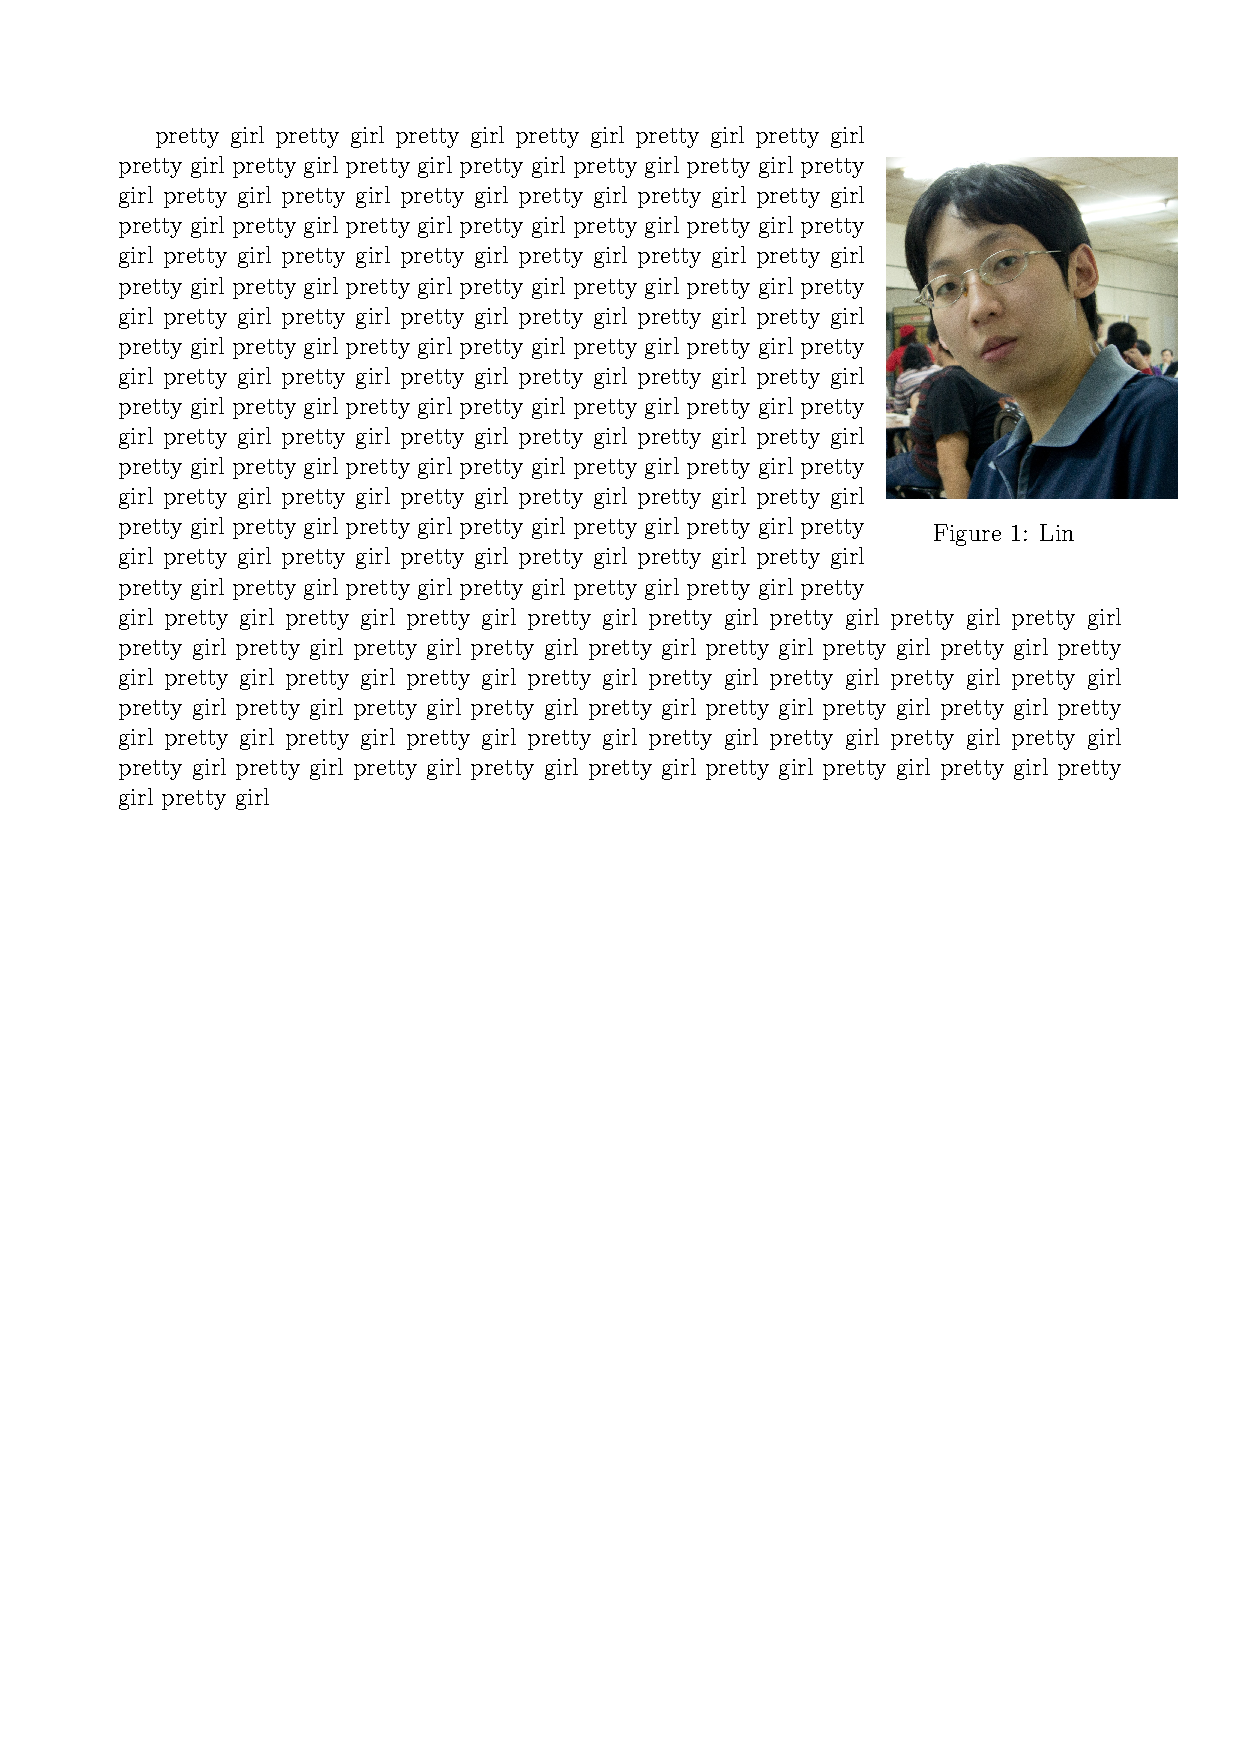
\includegraphics[scale=0.4]{./pics/wrap_figure.pdf} 
\end{minipage}% 
\begin{minipage}[b]{0.5\textwidth} 
\begin{footnotesize}
\begin{quote}
\begin{verbatim}
\usepackage{wrapfig}
\begin{wrapfigure}{r}{40mm}
\begin{center}
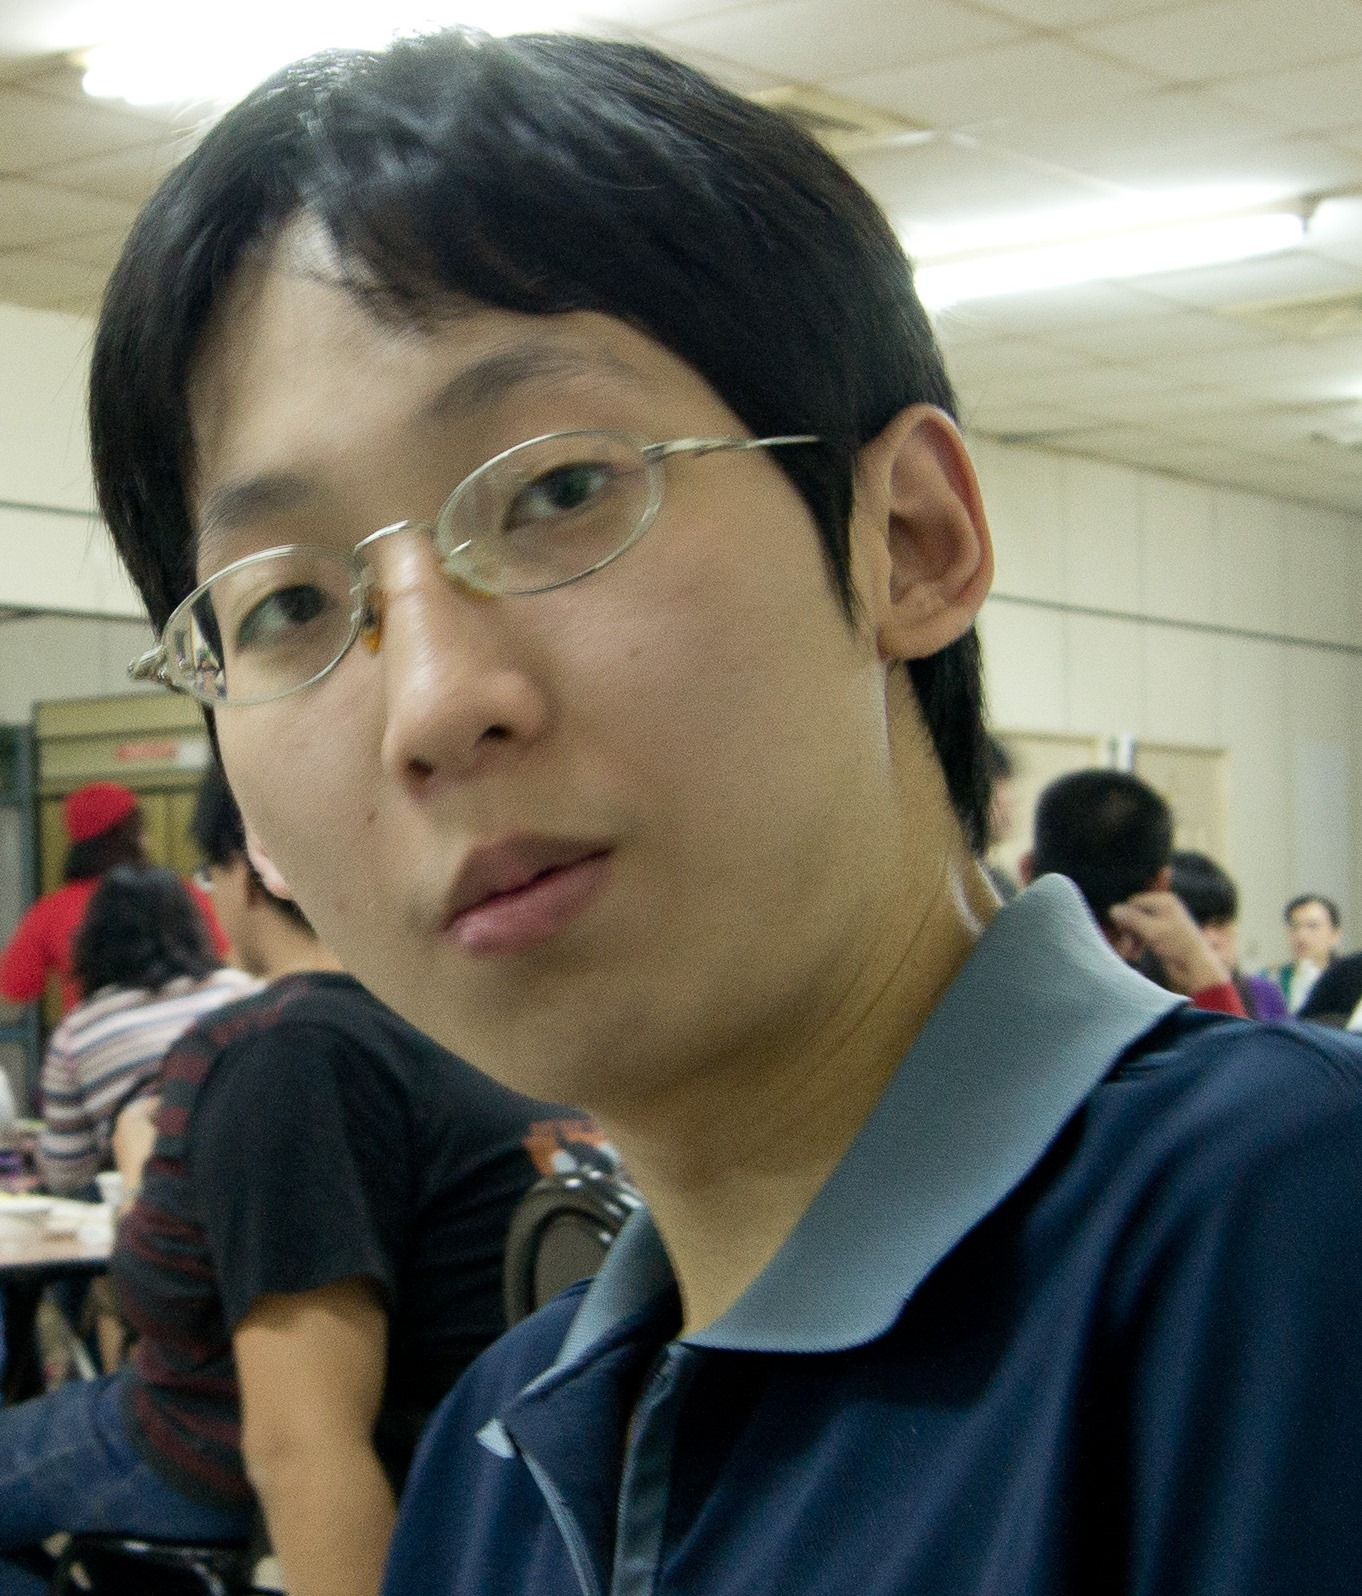
\includegraphics[scale=0.5]{./pics/lin.jpg}
\caption{Lin}
\end{center}
\end{wrapfigure}
\mbox{}
bla bla bla bla bla bla bla bla bla bla
\end{verbatim}
\end{quote}
\end{footnotesize}
\end{minipage} 
\caption{文繞圖範例}
\end{figure}
\vspace{-1cm}
\section{圖片尺寸大於文字邊界}
\vspace{-1cm}
\begin{figure}[!h] 
\begin{minipage}[b]{0.5\textwidth} 
\centering 
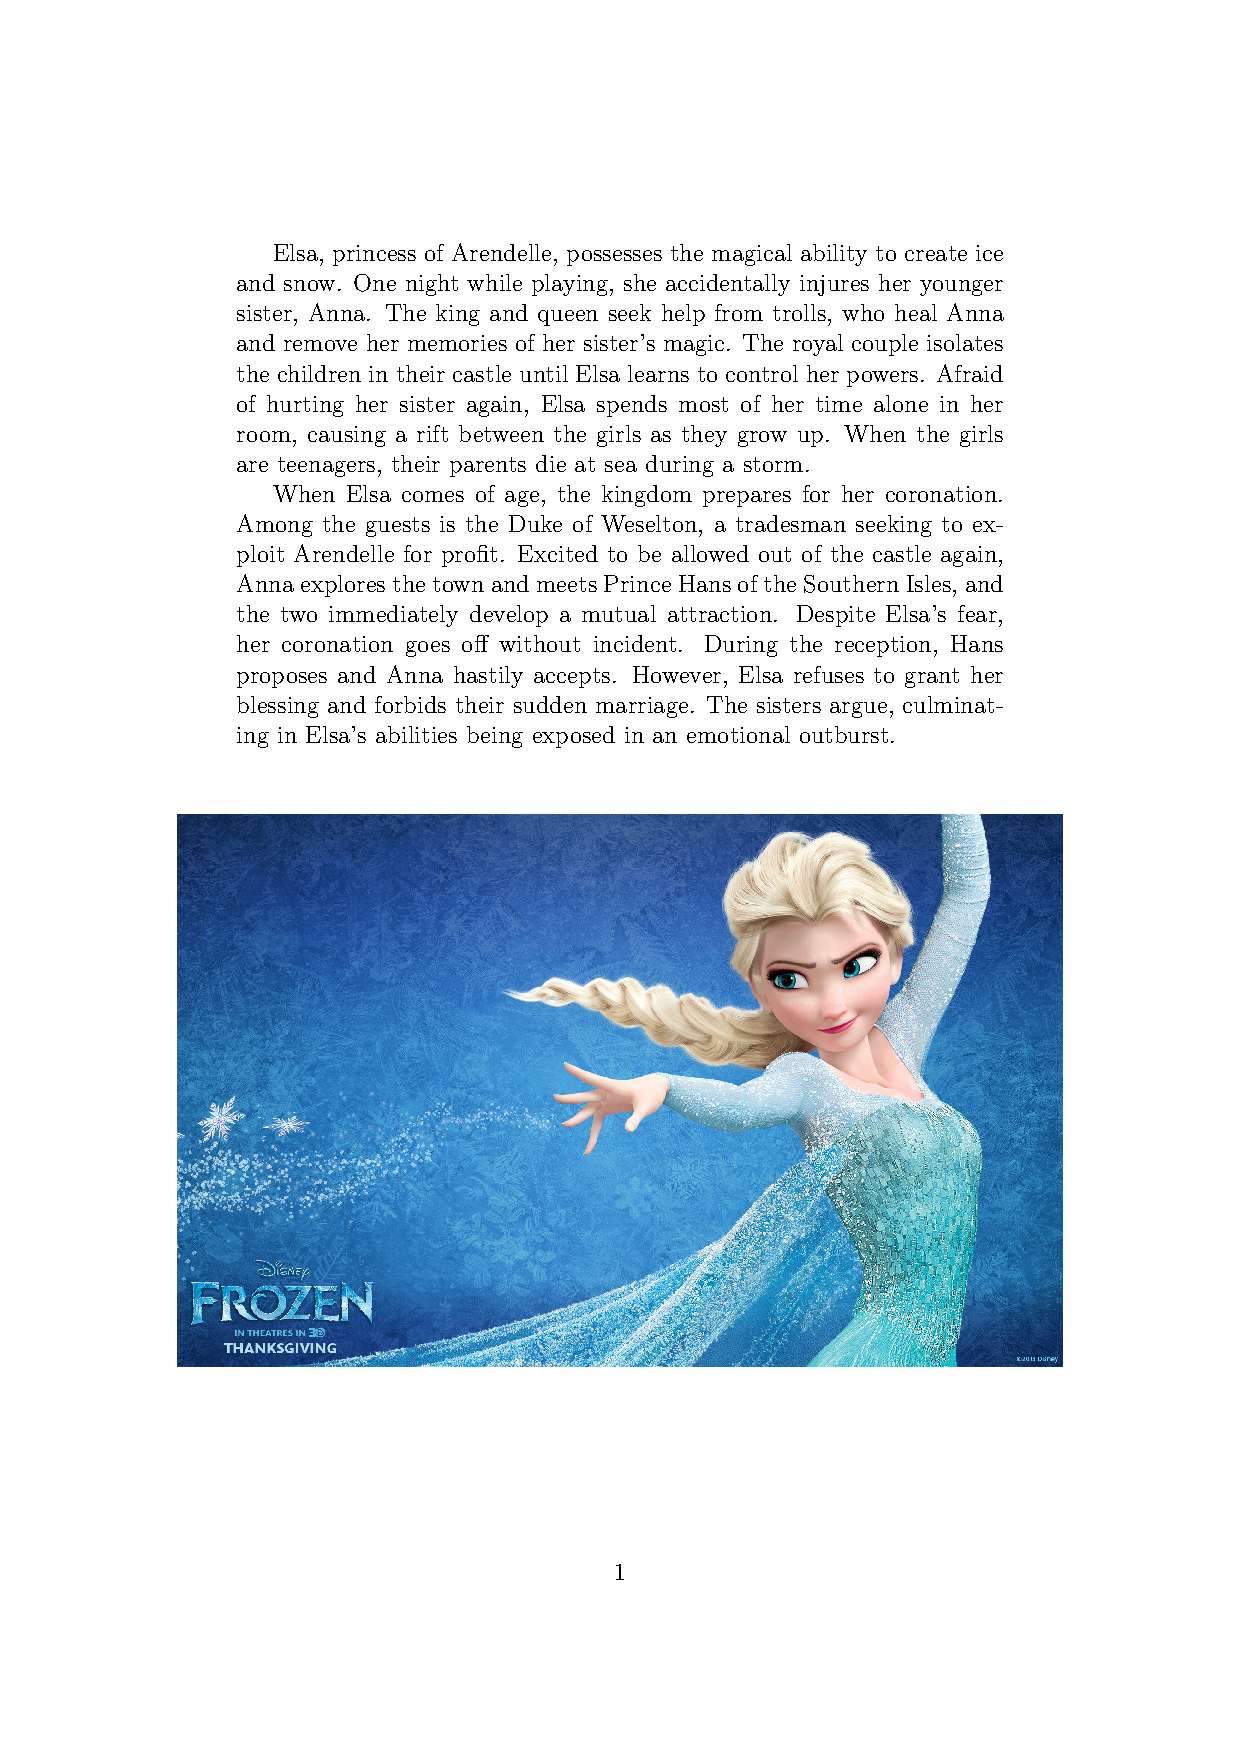
\includegraphics[scale=0.3]{./pics/figure_over_boundary_example.pdf} 
\end{minipage}% 
\begin{minipage}[b]{0.5\textwidth} 
\begin{footnotesize}
\begin{quote}
\begin{verbatim}
\usepackage[export]{adjustbox}
bla bla bla bla bla bla bla bla bla bla
\begin{figure}[!h]
\makebox[\textwidth][c]
{\raisebox{0pt}[10cm]
{
\includegraphics[width=15cm]{./pics/elsa.jpg}}}
\end{figure}

\end{verbatim}
\end{quote}
\end{footnotesize}
\end{minipage} 
\caption{圖片尺寸超出邊界}
\end{figure}

\newpage
\section{圖片旋轉}
\noindent 如果想要在latex中旋轉圖片,可以在設定圖片尺寸的地方再加上"angle"的指令就可以旋轉圖片了,在沒有指定旋轉中心的情況下,會針對圖片的左下角做旋轉,所以大家可以看到範例中的第三張圖片,轉-90度時,是以左下角為中心轉-90度,不過這並不是我們預想中的情況,所以只要加上固定旋轉中心的指令"origin=c"就可以讓圖以圖中心為圓心旋轉,轉-90度的情形就會變成第四張圖
\begin{figure}[!h] 
\begin{minipage}[b]{0.5\textwidth} 
\centering 
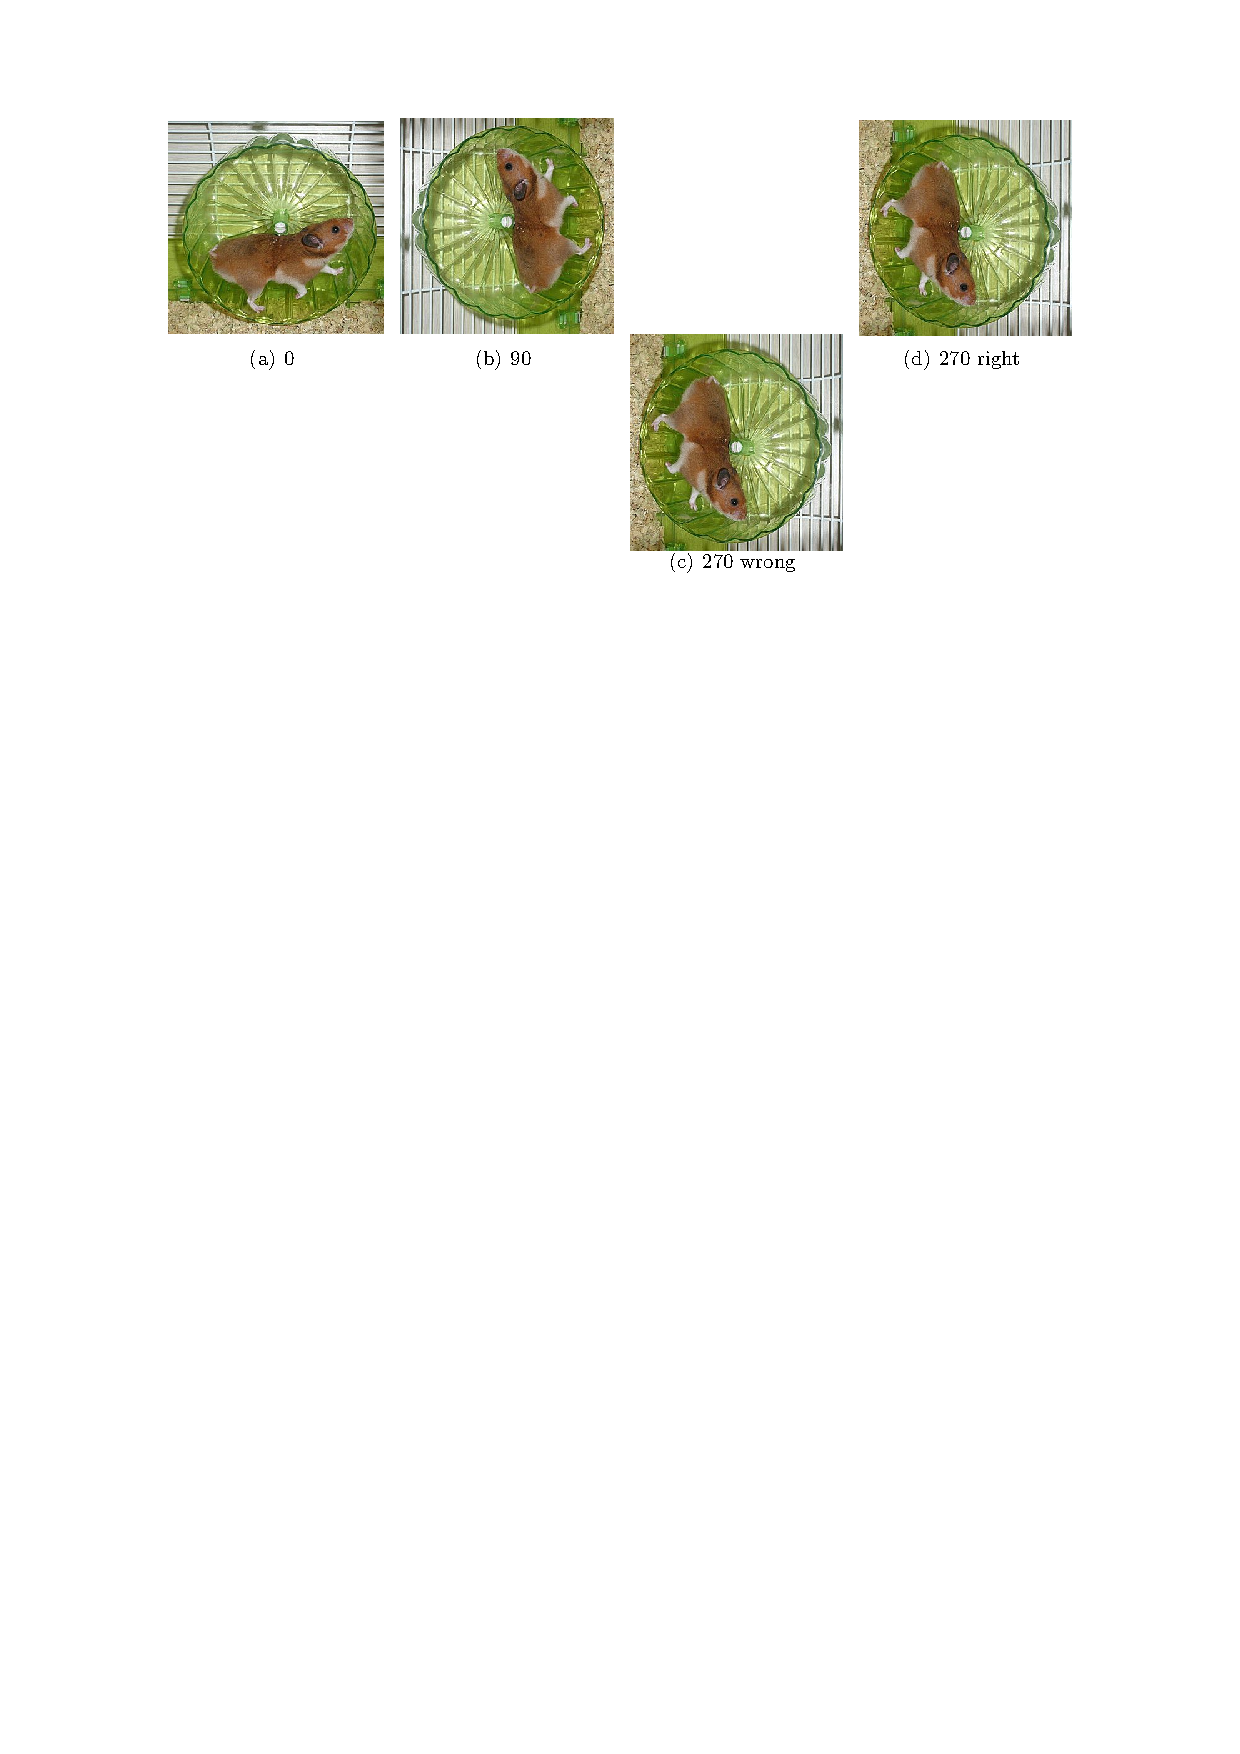
\includegraphics[scale=0.4]{./pics/rotate_example.pdf} 
\end{minipage}% 
\begin{minipage}[b]{0.5\textwidth} 
\begin{footnotesize}
\begin{quote}
\begin{verbatim}
\begin{figure}[!h]
\centering
\subfigure[0]{
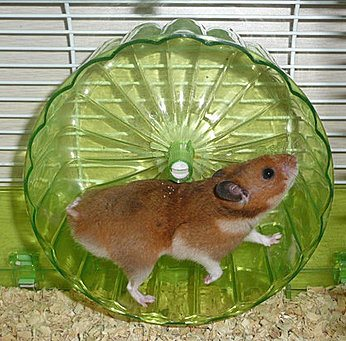
\includegraphics[scale=0.3,angle=0]
{mouse}}
\subfigure[90]{
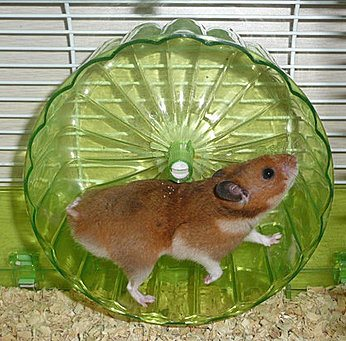
\includegraphics[scale=0.3,angle=90]
{mouse}}
\subfigure[270 wrong]{
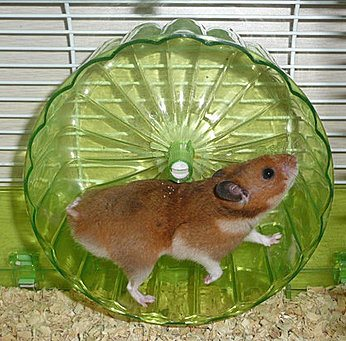
\includegraphics[scale=0.3,angle=-90]
{mouse}}
\subfigure[270 right]{
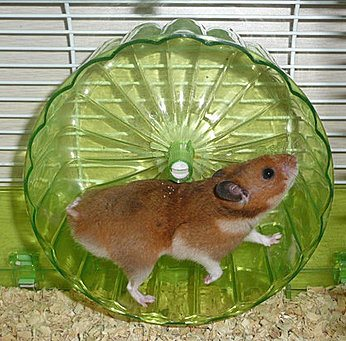
\includegraphics[origin=c,scale=0.3
,angle=-90]
{mouse}}
\end{figure}
\end{verbatim}
\end{quote}
\end{footnotesize}
\end{minipage} 
\caption{轉動圖片範例}
\end{figure}

\section{Subfigure v.s. Subfloat}
\noindent subfigure的用法已經在前面介紹過了,使用subfigure必須要用的是package subfigure,使用subfloat則是用package subfig,兩者不能同時存在,否則會導致錯誤
\begin{itemize}
\item subfloat用法
\begin{figure}[!h] 
\begin{minipage}[b]{0.5\textwidth} 
\centering 
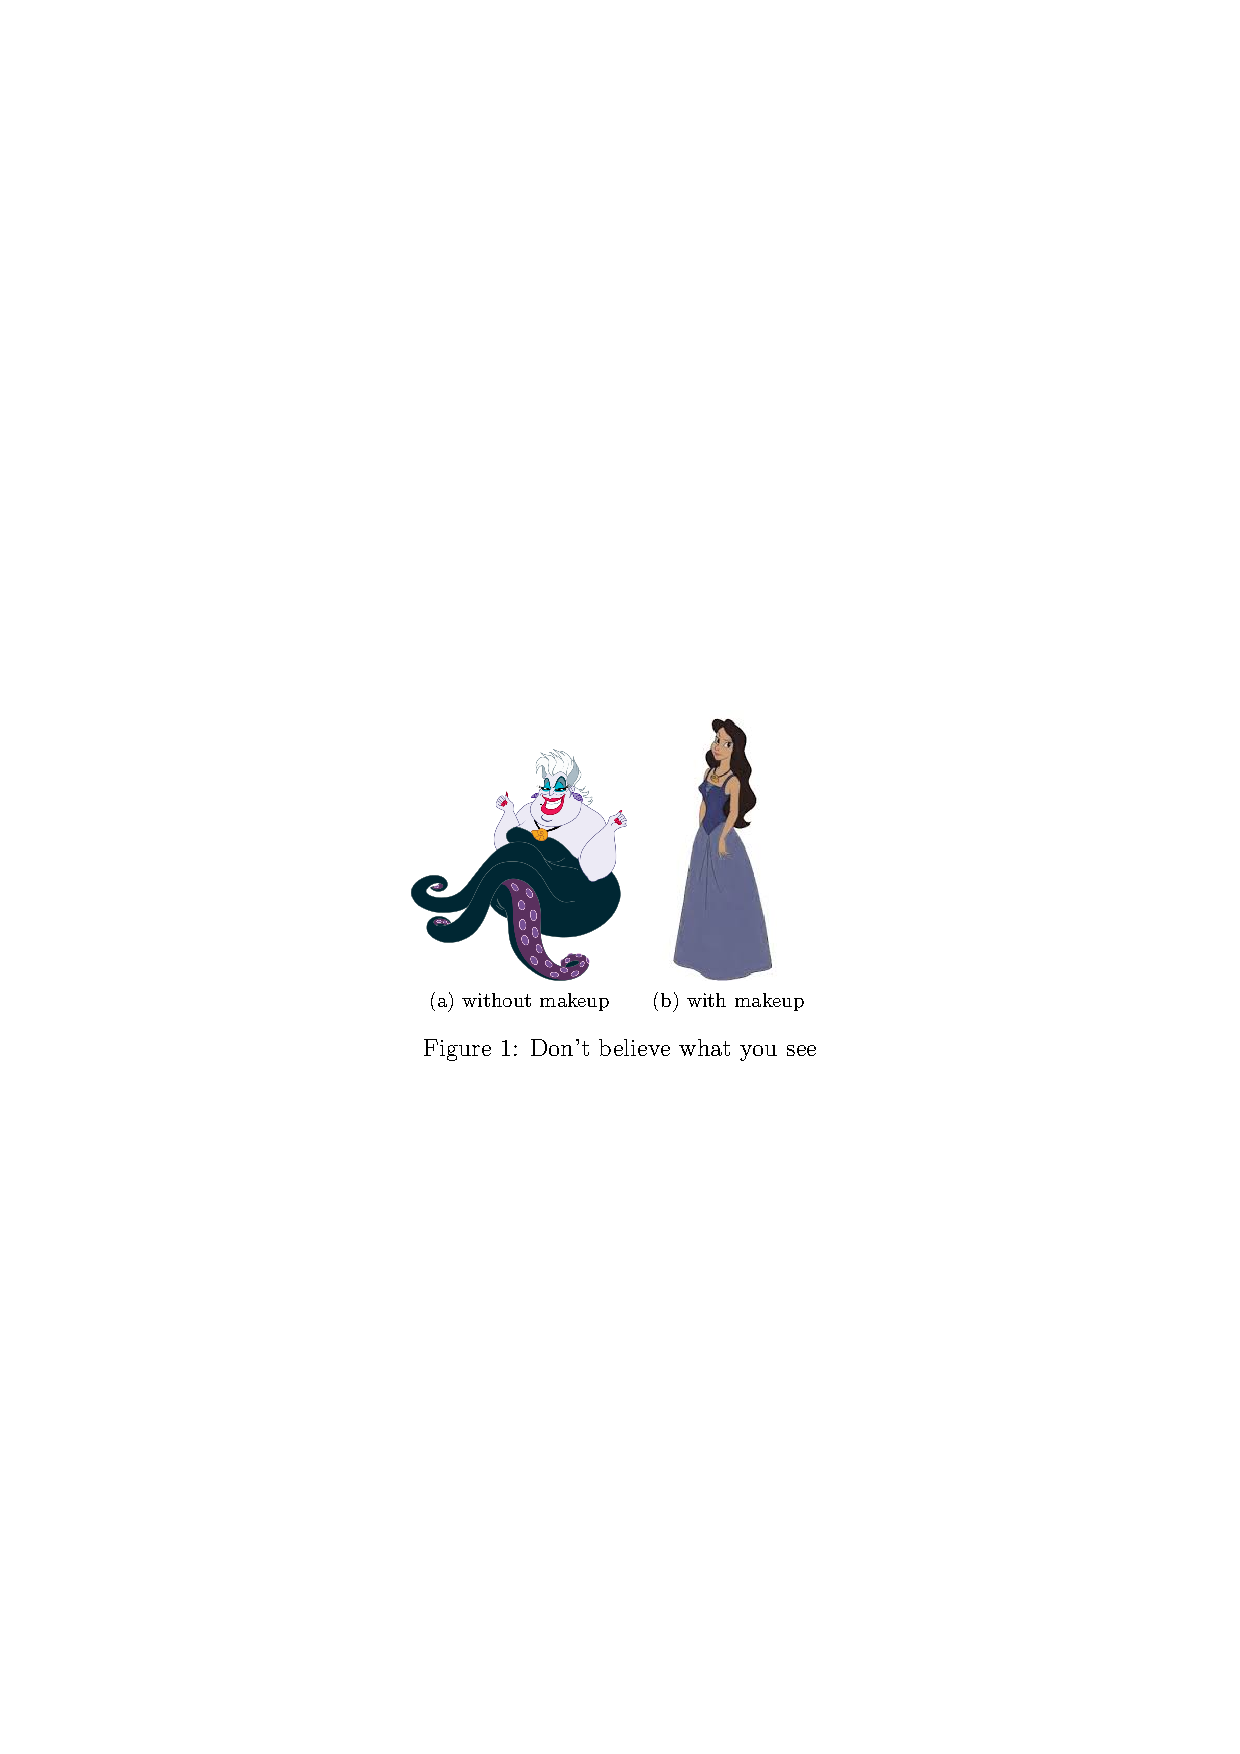
\includegraphics{./pics/subfloat_example.pdf} 
\end{minipage}% 
\begin{minipage}[b]{0.5\textwidth} 
\begin{footnotesize}
\begin{quote}
\begin{verbatim}
\begin{figure}
\centering
\subfloat[without makeup]{

\includegraphics[scale=0.5]{./pics/ursula_before.png}}
\subfloat[with makeup]{

\includegraphics[scale=0.5]{./pics/ursula_after.jpg}}
\caption{Don't believe what you see}
\end{figure}
\end{lstlisting}
\end{verbatim}
\end{quote}
\end{footnotesize}
\end{minipage} 
\caption{subfloat範例}
\end{figure}

除了所需要用到的package不一樣之外,上網搜尋過後,大致上是subfloat的性能優於subfigure,因為subfloat的可調參數比較多,不過一般我們在寫論文不太會用到這些參數設定,大家有興趣的話可以上網搜尋"The Subfig package"裡面有非常詳盡的介紹
\end{itemize}

\section{兩攔環境中圖置中}
\noindent 因為這個範例是要在兩欄的環境中進行,所以跟其他範例的環境設定是不一樣的(bla bla bla代表的是文章內容),其實要放一張橫越兩攔的圖只要在"figure"的後面加上*號就可以了,指令從"\textbackslash begin \{figure\}"變成"\textbackslash begin \{figure*\}",不過目前嘗試無法控制圖片的位置,範例中的圖片會自動跑到第二頁無法控制讓圖片顯示在第一頁
\begin{figure}[!h] 
\begin{minipage}[b]{0.5\textwidth} 
\centering 
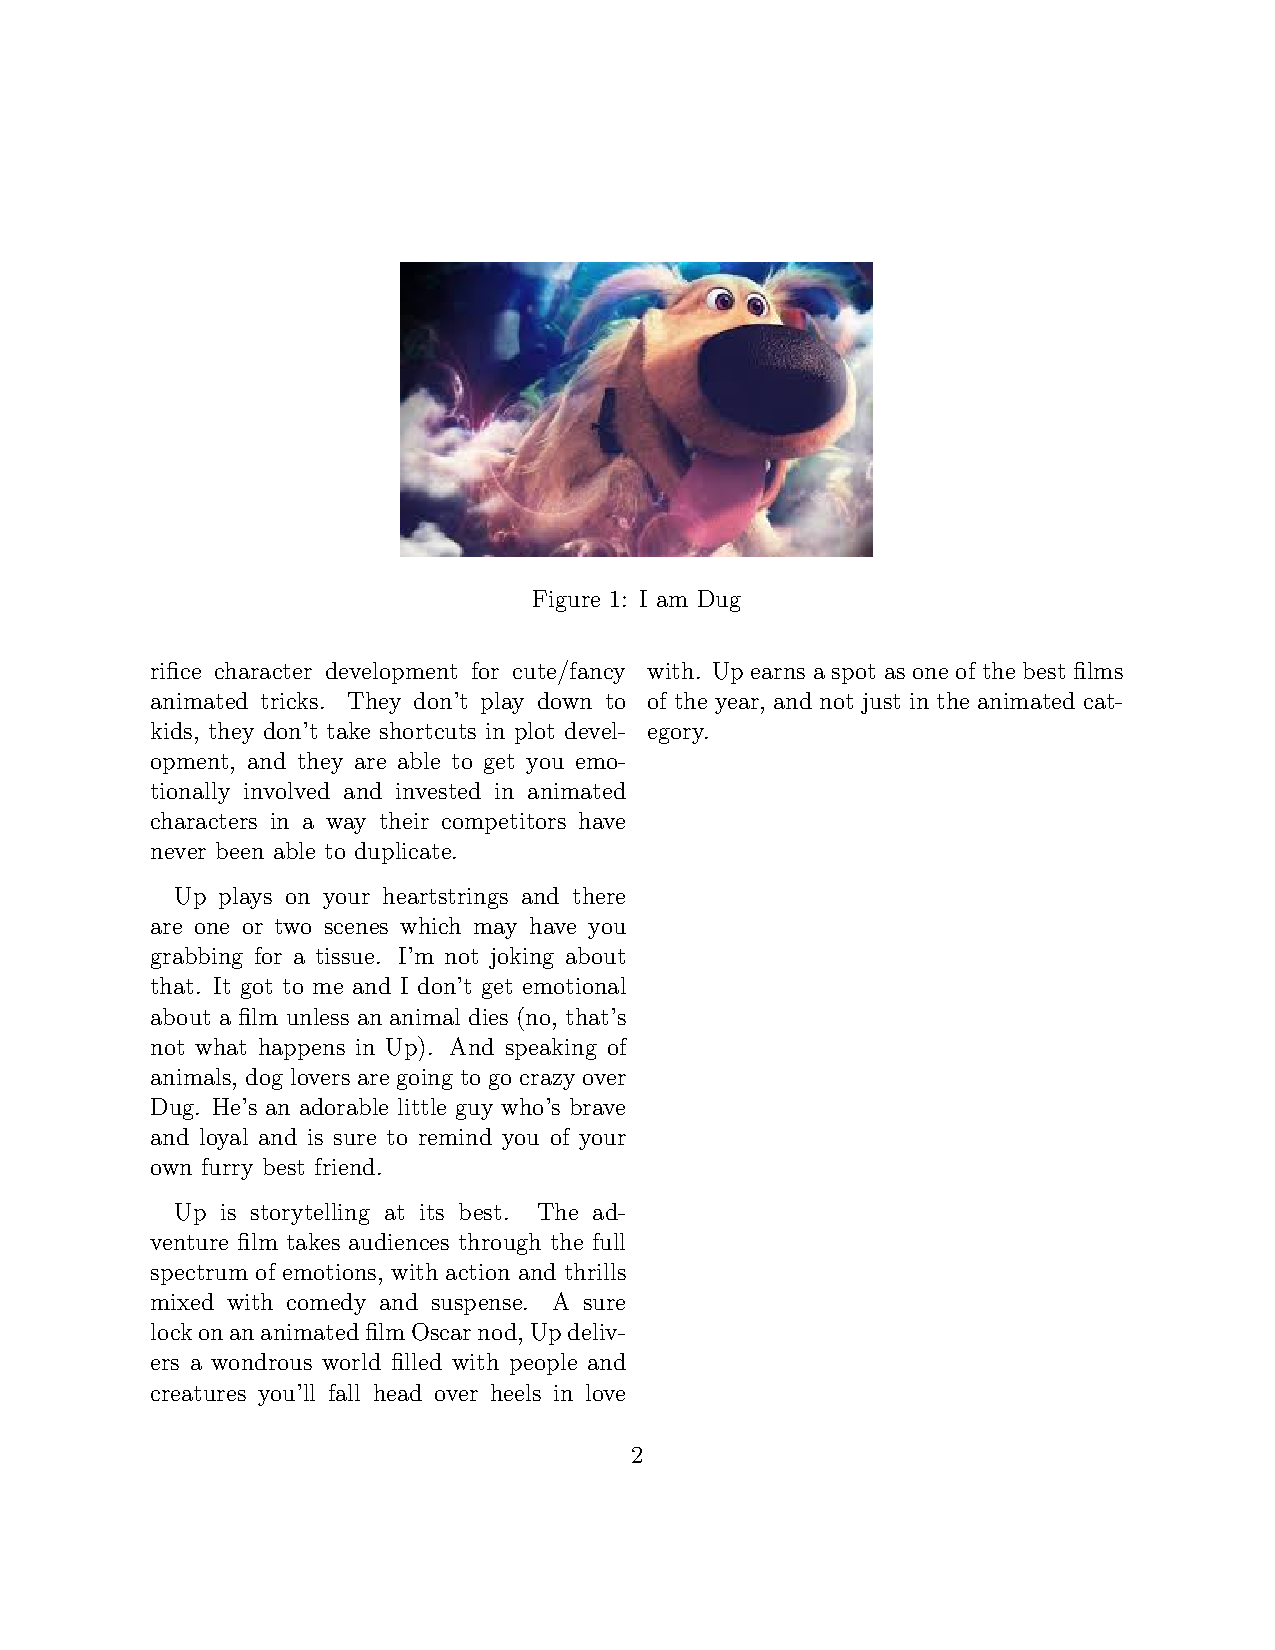
\includegraphics[scale=0.3]{./pics/twocolumn_figure_example.pdf} 
\end{minipage}% 
\begin{minipage}[b]{0.5\textwidth} 
\begin{footnotesize}
\begin{quote}
\begin{verbatim}
bla bla bla bla bla bla bla
\begin{figure*}[htb]
\centering

\includegraphics[width=8cm]{./pics/dog.jpg}
\caption{I am Dug}
\end{figure*} 
bla bla bla bla bla bla bla
\end{verbatim}
\end{quote}
\end{footnotesize}
\end{minipage} 
\caption{兩攔環境下的大圖}
\end{figure}


\section{適當的圖文比例}
\begin{itemize}
\item 標題要清楚明瞭
\item 圖表所包含的每一個因素都要標明清楚
\item 圖表是一個獨立的概念,必須完整
\item 不要濫用圖表

\end{itemize}




\clearpage
\end{CJK}
\end{document}
